 \chapter{BaseLib Level 1}
\chaptermark{Level 1}

BaseLib Level1 group togheter differents BaseLib data structures that are vital for each application developed on the library. The first component this chapter deal with is the \textit{Object Registry Database} (ORDB) a data structure that let the user query about the run time type identification of an object (something similar with the C++'s RTTI infrastructure addressed below).
Another really usefull infrastructure is the \textit{Global Object Database} (GODB) a database structure that holds a reference to each instantiated class and also let it be garbage collectable. An \textit{Error System Instruction} is partially introduced as a linked list stucture. In Level1 you are going to see for the first time the foundamental \textit{Configuration Database}, a tree data structure that holds the most important information for the loading and configuration of the system. In such level it also possible to find the file \texttt{StreamAttributes.h} that defines some attributes that concern streams, such file will be not addressed in the following.


Classes in BaseLib Level1 can be grouped with the following criteria:
\begin{itemize}
 \item Object Registry DataBase (ORDB)
 \item Global Object DataBase (GODB)
 \item Error System Instruction (ESI)
 \item Configuration DataBase (CDB)
 \item Stream Attributes
\end{itemize}
Such groups cover all BaseLib Level 1 classes, we start analysing the first group.



\section{Object Registry DataBase}
Before starting to introduce the Object Registry DataBase structure we spend some words trying to create a general basic knowledge about Object Oriented Languages and Run Time Type Identification. RTTI, i.e. Run-Time Type Information, or Run-Time Type Identification, refers to a C++ system that keeps information about an object's data type in memory at runtime. Run-time type information can apply to simple data types, such as integers and characters, or to generic objects. This is a C++ implementation of a more generic concept called reflection.



\subsection{RTTI}

Run Time Type Identification provides some information about objects at run time such as the name of its type. The C++ language has RTTI support, which fulfills the minimal requirements, but it is not enough for many applications of RTTI, such as object persistency. Other languages (like Java and C\#) have better RTTI system making possible to declare properties for accessing the objects and the language implements also persistency (serialization in Java), but these languages have other disadvantages.

C++ programs may also need persistency and the advanced features of RTTI systems. The C++ language is so powerful that it is possible to implement properties and an advanced RTTI system.\\


The standard C++ provides the \texttt{typeid()} operator for getting type information. Its argument is an expression (a reference or a pointer of an object) or a type name. It returns a constant reference to a \texttt{type\_info} object containing some information of the object's type.

The \texttt{type\_info} class has only a few member functions:
\begin{lstlisting}[
extendedchars=true,%
basicstyle=\fontfamily{pcr}\fontseries{m}\selectfont\footnotesize, %
stepnumber=1,%
numberstyle=\tiny,%
keywordstyle=\footnotesize\tt ,%
language=C++]
class type_info {
public:
  virtual ~type_info();
  bool operator== (const type_info& rhs) const;
  bool operator!= (const type_info& rhs) const;
  bool before (const type_info& rhs) const;
  const char* name() const;
private:
  type_info (const type_info& rhs);
  type_info& operator= (const type_info& rhs);
};
\end{lstlisting}

The method \texttt{name} gets the string representation of the type (e.g. \texttt{int}, or \texttt{MyClass}); \texttt{before} is used for ordering; \texttt{operator==()} and \texttt{operator!=()} for comparing \texttt{type\_info} objects; this information does not help to find the relations of objects and does not solve most of the problems that arise in applications. It is not designed for that. All applications have different requirements and the same standard type description cannot fulfill all the requirements. \\


However the \texttt{type\_info} class can be used as a key in a map storing more detailed type information [Strousstrup 15.4.4]. This way every application can define and use its own RTTI system, which is a very flexible solution. The problem is, that someone has to define the structure of the RTTI record and fill the map with records for every type. This job is not trivial and some code has to be written for every application for doing that. \\


An alternative to this problem could be to write a piece of code able to walk the RTTI structure builded by the C++ compiler. RTTI data structures are necessary at run time for the \textit{dynamic cast} process; but what happens is that every compiler, developed from different companies, has its own data structures that differ from product to product. Using such strategy it is possible to exploit compile time produced data structures without creating your own data structures, i.e. having two parallels RTTI tables. \\



\subsection{ORDB}
BaseLib addresses the problem of knowing every class in the system holding an ORDB that is a simple linked list of all class types loaded in the system. There is only one instance of an ORDB (of type \texttt{ObjectRegistryDataBase}) at runtime and is called \texttt{ObjectRegistryDataBaseInstance} (see file \textit{level1/ObjectRegistryDataBase.cpp}). \\


The ORDB doesn't hold the hierarchy relationship between classes but it's only a list of all class types registered in the system, this list can be searched for a class by name or by an id number and it is possible to retrieve the name address of the class and other usefull informations. The whole structure of all classes that makes the ORDB work is depicted in Figure \ref{f:level1:object} that follows.

\begin{figure}[h!]
 \begin{center}
  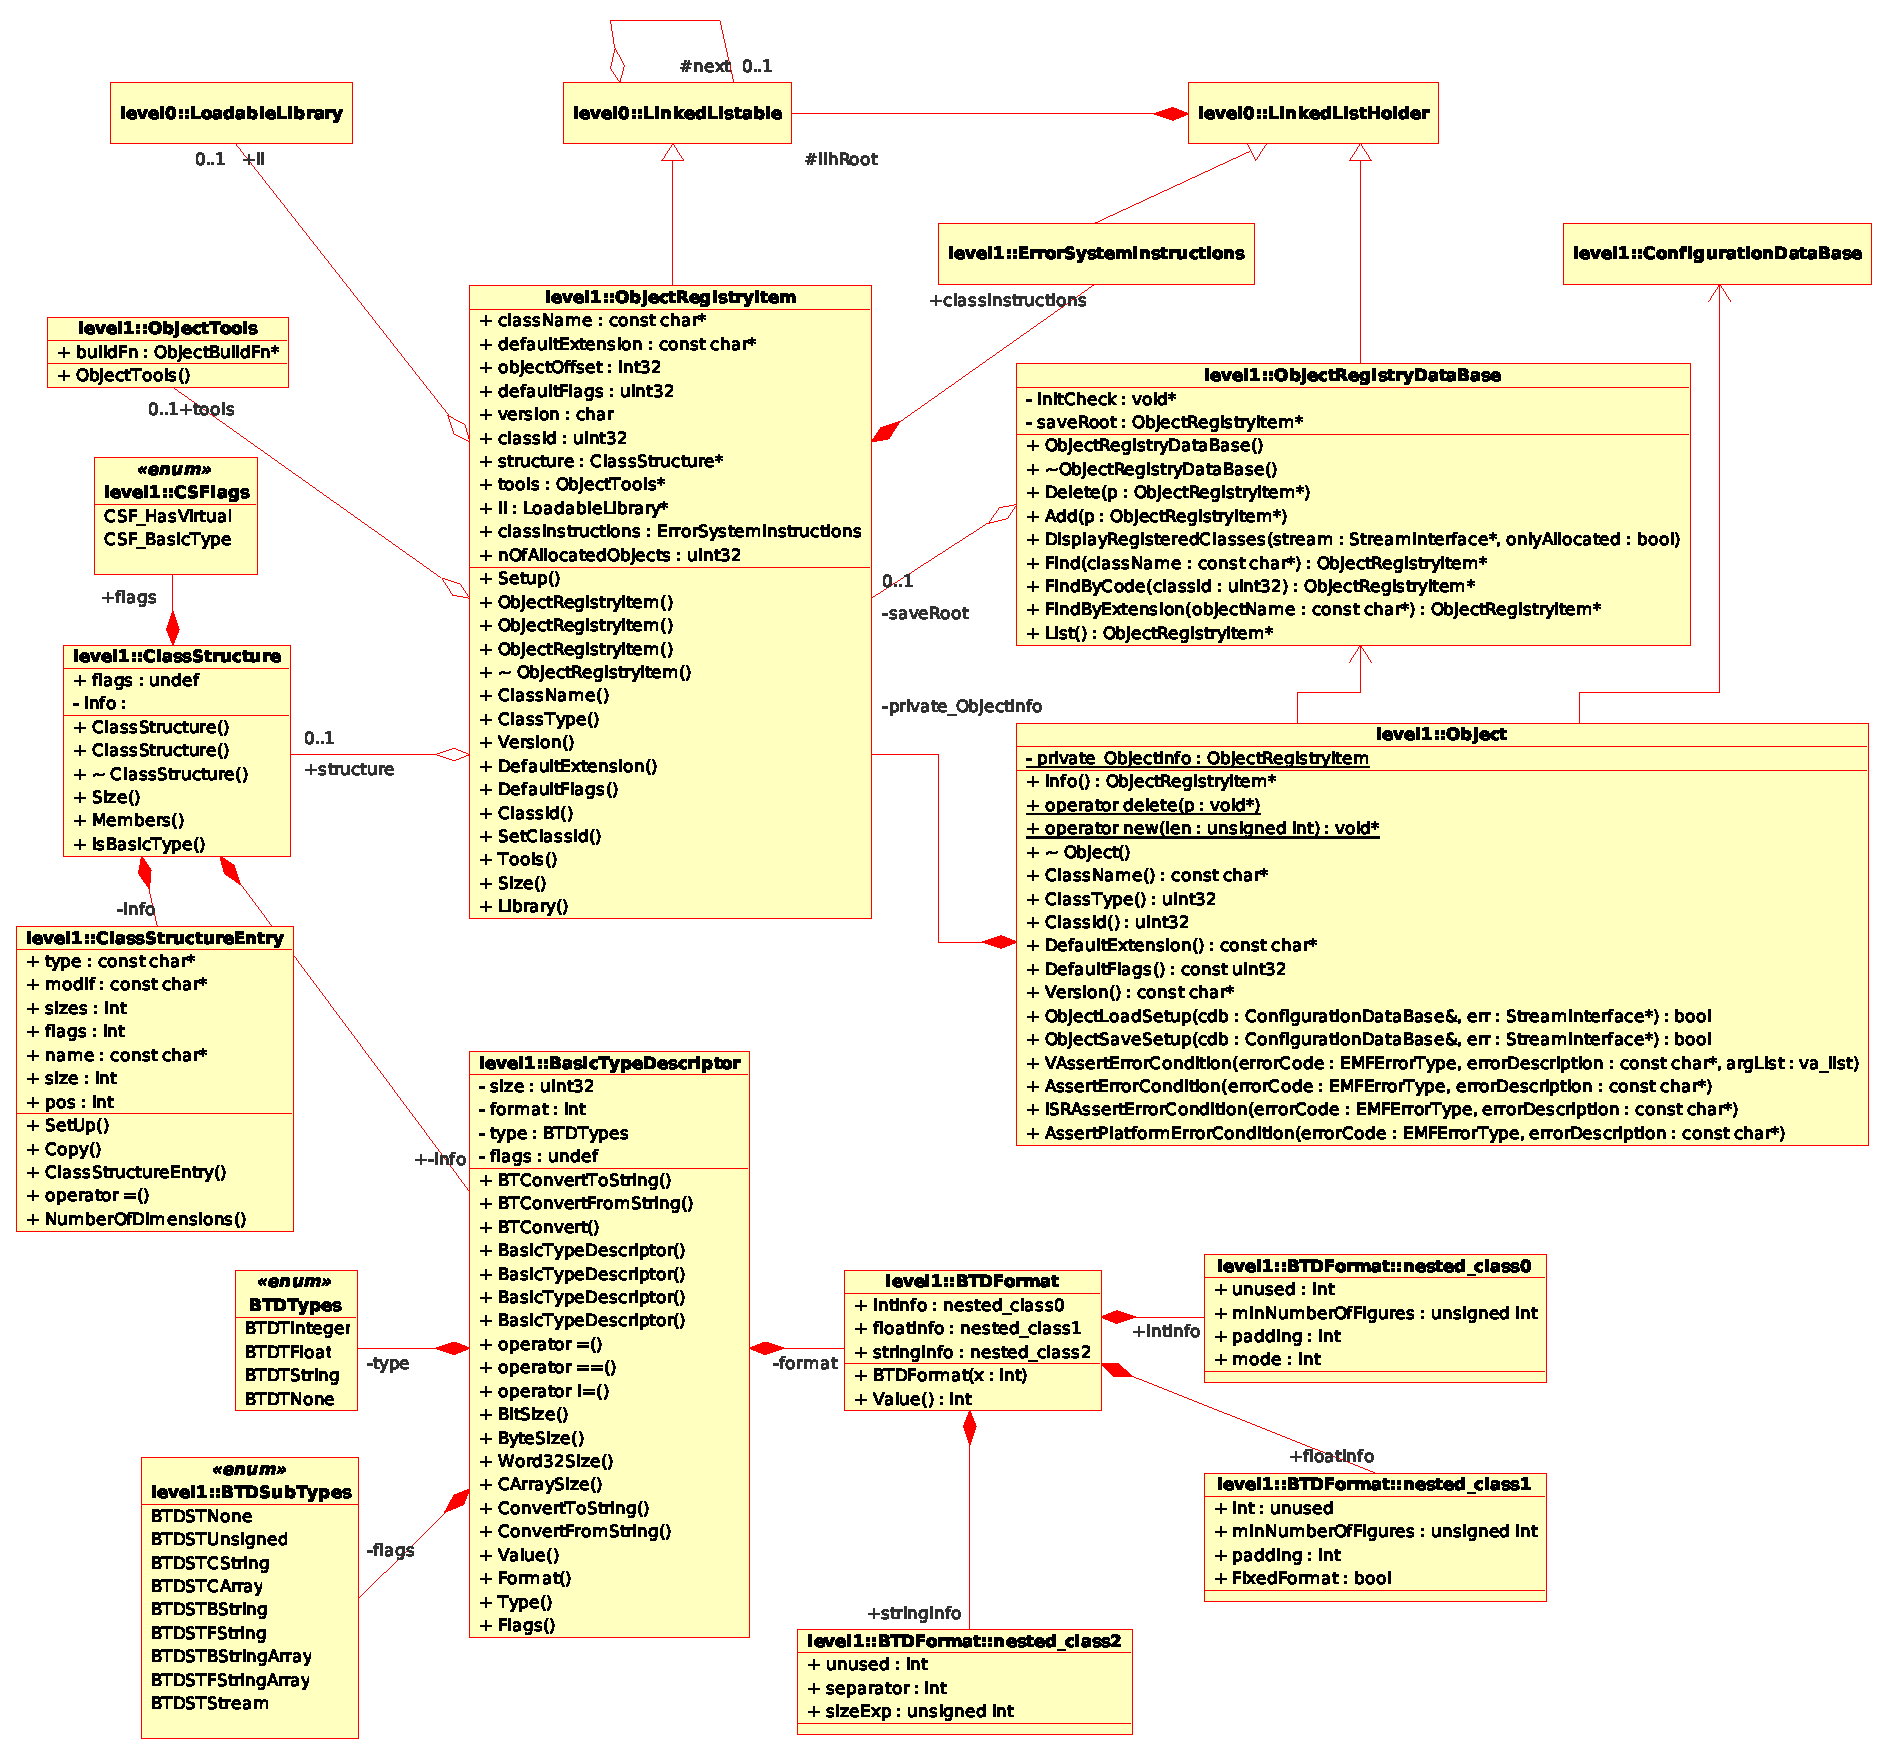
\includegraphics[width=\textwidth]{level1/level1-object.eps}
  \caption{BaseLib Level1 Object Registry Database (ORDB) classes}
  \label{f:level1:object}
 \end{center}
\end{figure}

Classess that belong to this group are:
\begin{itemize}
 \item ClassStructureEntry
 \item ClassStructure

 \item BasicTypeDescriptor
 \item BTDFormat

 \item ObjectRegistryItem, ObjectTools
 \item ObjectRegistryDataBase
 \item Object
\end{itemize}

All classes listed above estabilsh the \textit{Object Registry Database} structure. The basic idea behind this work is to imitate what is developed in the Java language: every object inherit from the \texttt{Object} class providing a common ancestor of every object that force to have some common methods (like \texttt{ToString} in Java).
In BaseLib we want to achieve the same common ancestor letting all the objects inheriting common methods and common functionalities like the most important one: be part of the ORDB. Such ORDB can be easily walked by any other object providing debbugging functionalities and runtime linking and loading. \\


We first go throught the implementation of the \texttt{ObjectRegistryDataBase} and then we show how the class \texttt{Object} can take advantage of it and which basic methods add to any other objects that inherith from that. We start with some utility classes.



\subsubsection{BTDFormat}
\texttt{[BasicTypes.h]}\\
Class \textbf{BTDFormat} is declared as a \texttt{union} with a constructor and a single method \texttt{Value}. Attribute can be a \texttt{struct intInfo}, \texttt{struct floatInfo} or \texttt{struct stringInfo}. Each struct, that follows, try to describe the format of a single basic type that can be \textit{integer}, \textit{float} or \textit{string}. The format of the \texttt{BTDFormat} depends on the endianity so that to fit in the 14 bit space in the \textbf{BasicTypeDescriptor} attribute's \texttt{format} analized in the next section.

\begin{lstlisting}[
extendedchars=true,%
basicstyle=\fontfamily{pcr}\fontseries{m}\selectfont\footnotesize, %
stepnumber=1,%
numberstyle=\tiny,%
keywordstyle=\footnotesize\tt ,%
language=C++]
union BTDFormat {
   struct {
      unsigned int minNumberOfFigures:5;
      int padding:3;
      int mode:3;
      int unused: 21;
   } intInfo;
   struct {
      unsigned int minNumberOfFigures:5;
      int padding:3;
      bool fixedFormat:1;
      int unused: 23;
   }floatInfo;
   struct {
      int separator:3;
      unsigned int sizeExp:4;
      int unused: 25;
   } stringInfo;

   BTDFormat(int x=0);
   int Value();
};
\end{lstlisting}

\texttt{intInfo} is used in single strings and streams, \texttt{floatInfo} is used in floats to determine how many meaningful figures are there and \texttt{stringInfo} is used in strings of C ARRAYs and BSTRING type.



\subsubsection{BasicTypeDescriptor}
\texttt{[BasicTypes.h, BasicTypes.cpp]}\\

Support for basic types of built in language types. Each basic type is described in BaseLib with a \texttt{BasicTypeDescriptor}, such class has the following attributes that account about the size of the object, attribute \texttt{size}, maximum size is 1024 units (10 bit), the format and type.

\begin{lstlisting}[
extendedchars=true,%
basicstyle=\fontfamily{pcr}\fontseries{m}\selectfont\footnotesize, %
stepnumber=1,%
numberstyle=\tiny,%
keywordstyle=\footnotesize\tt ,%
language=C++]
private:
   uint32 size:10;
   int format:14;
   BTDTypes type:4;
   BTDSubTypes flags:4;
\end{lstlisting}

Actually a \texttt{BasicTypeDescriptor} describes a basic type with a \texttt{type} and a \texttt{subtype}, so we have a two level description. The first level (\texttt{enum BTDTypes}) discriminate about:
\begin{itemize}
 \item \texttt{BTDTInteger}, an integer;
 \item \texttt{BTDFloat}, standard float;
 \item \texttt{BTDString}, any type of string;
 \item \texttt{BTDTNone} that's denote not a \texttt{BTDType};
\end{itemize}

For some of that specifiers there is a more precise description thanks to the \texttt{enum BTDSubType}, note that in the source code there is no \texttt{enum BTDSubType} but can be a good idea to make it. The \texttt{BTDSubType flag} define the meaning of the \texttt{size} attribute.
\begin{itemize}
 \item \texttt{BTDSTNone} no flags;
% FLAGS relative to BTDTInteger
 \item \texttt{BTDSTUnsigned} modifier for the integer;
% FLAGS relative to BTDTString
 \item \texttt{BTDSTCString} the \texttt{void*} is casted to \texttt{char**}; it's assumed to be a vector of pointers of \texttt{size} matching     that of the source, when used as destination the existing pointer is first freed and then replaced with a new malloced one;
 \item \texttt{BTDSTCArray} \texttt{char[]}, \texttt{size} field is the array size, the string is always 0 terminated;
 \item \texttt{BTDSTBString} \texttt{BString} class, \texttt{size} field is meaningless \texttt{void*} is \texttt{BString*} it is a pointer to a single \texttt{BString} the parts will be separarted using the character specified in the format field;
 \item \texttt{BTDSTFString} \texttt{FString} class, \texttt{size} field is meaningless \texttt{void*} is \texttt{FString*} it is a pointer to a single \texttt{FString} the parts will be separated using the character specified in the format field;
 \item \texttt{BTDSTBStringArray} \texttt{BString} class, \texttt{size} field is meaningless \texttt{void*} is \texttt{BString*} it is an array of \texttt{BString}s matching the input size;
 \item \texttt{BTDSTFStringArray} \texttt{FString} class, \texttt{size} field is meaningless \texttt{void*} is \texttt{FString*} it is an array of \texttt{FString}s matching the input size;
 \item \texttt{BTDSTStream} \texttt{StreamInterface} class, \texttt{size} field is meaningless.
\end{itemize}

A complete picture of that hierarchy is showed in Figure \ref{f:level1:BasicTypes}. It is really important to note the relationship between those types.
\begin{figure}[h!]
 \begin{center}
  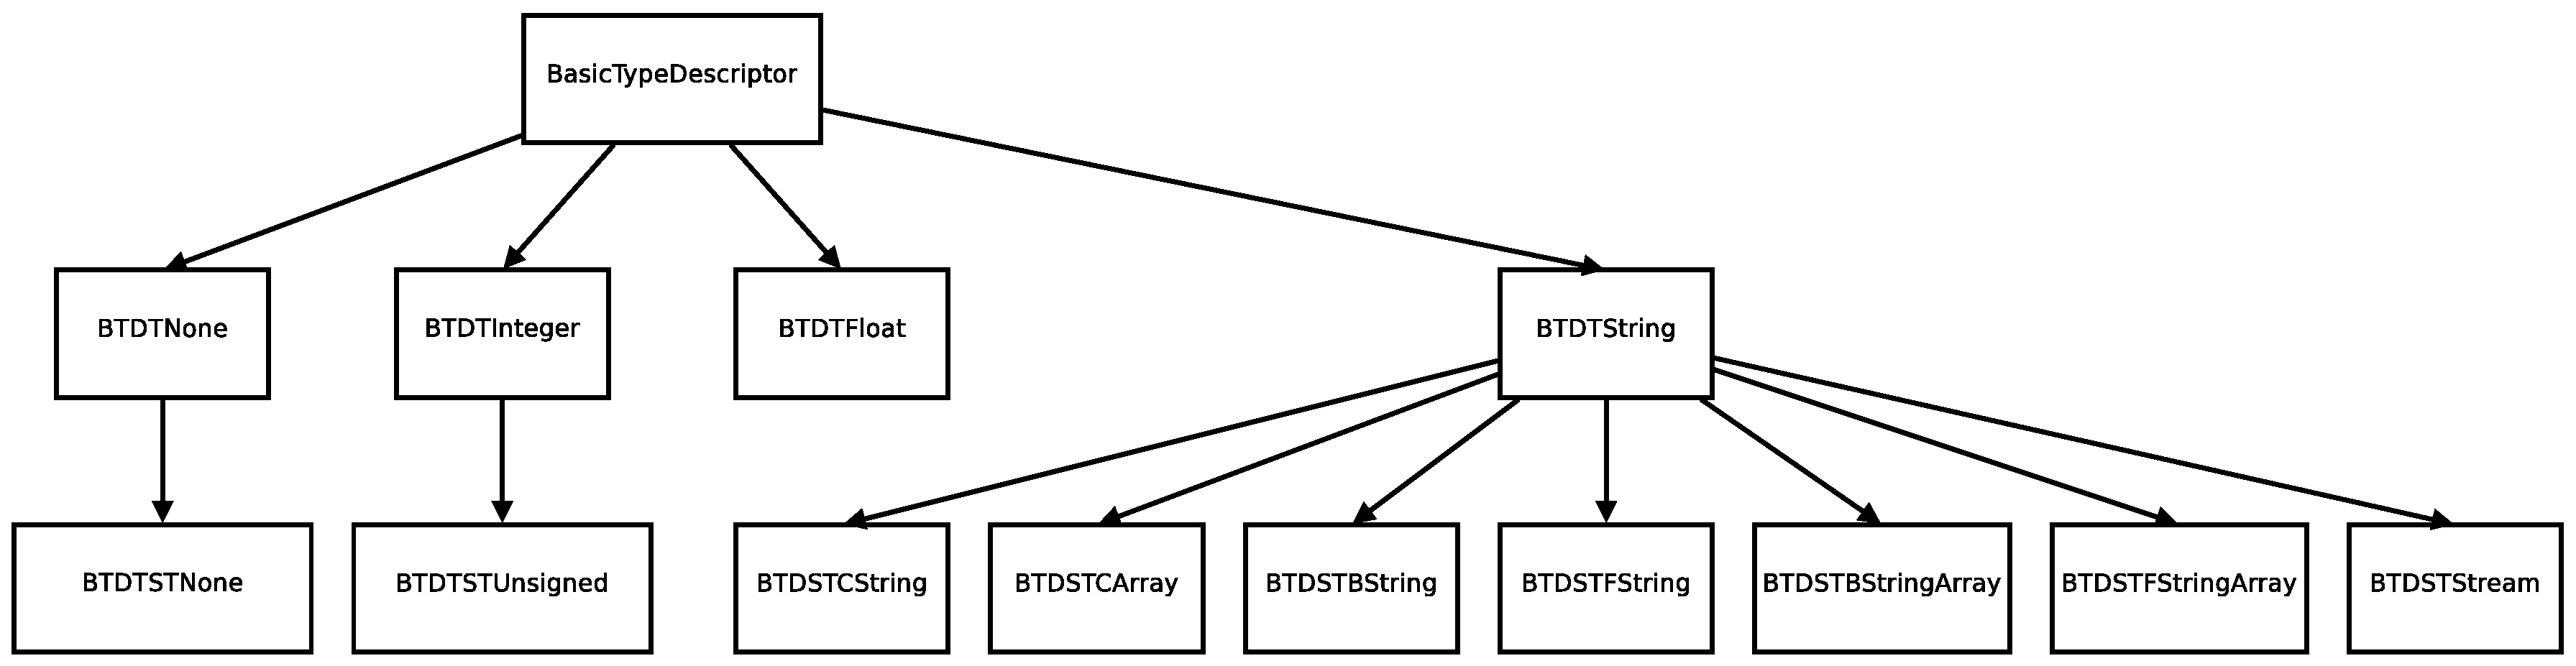
\includegraphics[width=\textwidth]{level1/types.eps}
  \caption{BaseLib Level1 BasicTypes hierarchy}
  \label{f:level1:BasicTypes}
 \end{center}
\end{figure}

Now we take a look to the methods exported from such class, there are four constructors, the first one create a \texttt{BasicTypeDescriptor} with \texttt{size} 32 bit, \texttt{type} \texttt{BTDTInteger}, \texttt{flags} \texttt{BTDSTNone} and \texttt{format} \texttt{NULL}, so it makes a \texttt{BasicTypeDescriptor} of an \textit{int32}. The second constructor helps making a new object using another one via the method \texttt{Value}. The third constructor is the most used in the library it let you construct your own basic type by setting each attribute in the class. The comes the copy constructor. \\


Then comes some getter methods that returns the size of the basic type counting the bits, bytes abd words (\texttt{BitSize}, \texttt{ByteSize} and \texttt{Word32Size} that is the minimum number of words to hold it); \texttt{CArraySize} is the size of a \texttt{CArray}. The method \texttt{Value} convert a \texttt{BasicTypeDescriptor} in an integer, \texttt{Format} return the \texttt{format} attribute, \texttt{Type} return the \texttt{type} attribute and \texttt{Flags} the \texttt{flags} attribute. \\


Methods \texttt{ConvertToString} and \texttt{ConvwertFromString} convert a string like ``uint'' in a \texttt{BasicTypeDescriptor} of type \texttt{BTDTInteger} and subtype \texttt{BTDSTUnsigned} and back.


\begin{lstlisting}[
extendedchars=true,%
basicstyle=\fontfamily{pcr}\fontseries{m}\selectfont\footnotesize, %
stepnumber=1,%
numberstyle=\tiny,%
keywordstyle=\footnotesize\tt ,%
language=C++]
public:
   BasicTypeDescriptor();
   BasicTypeDescriptor(int32 equivalent);
   BasicTypeDescriptor(uint32 size,BTDTypes type, BTDSubTypes flags,BTDFormat format = BTDFNone);
   BasicTypeDescriptor(const BasicTypeDescriptor& desc);
   BasicTypeDescriptor operator=(const BasicTypeDescriptor &desc);

   bool operator==(const BasicTypeDescriptor &desc) const;
   bool operator!=(const BasicTypeDescriptor &desc) const;

   int32 BitSize() const;
   int32 ByteSize() const;
   int32 Word32Size() const;
   uint32 CArraySize() const;

   int32 Value() const;
   BTDFormat Format() const;
   BTDTypes Type() const;
   BTDSubTypes Flags() const;

   const char* ConvertToString(BString& string) const;
   bool ConvertFromString(const char* name);
\end{lstlisting}

In the file \textit{level1/BasicTypes.h} are declared the following basic type descriptors, with the following parameters.
\begin{table}[!h]
 \begin{center}
  \begin{tabular}{|lllll|}
   \hline
type & BaseLib type & bit size & \texttt{BTDTypes} & \texttt{BTDSubTypes} \\
   \hline
8 bit signed integer & \texttt{BTDInt8} & 8 & BTDTInteger & BTDSTNone \\
16 bit signed integer & \texttt{BTDInt16} & 16 & BTDTInteger & BTDSTNone \\
32 bit signed integer & \texttt{BTDInt32} & 32 & BTDTInteger & BTDSTNone \\
64 bit signed integer & \texttt{BTDInt64} & 64 & BTDTInteger & BTDSTNone \\
8 bit unsigned integer & \texttt{BTDUint8} & 8 & BTDTInteger & BTDSTUnsigned \\
16 bit unsigned integer & \texttt{BTDUint16} & 16 & BTDTInteger & BTDSTUnsigned \\
32 bit unsigned integer & \texttt{BTDUint32} & 32 & BTDTInteger & BTDSTUnsigned \\
64 bit unsigned integer & \texttt{BTDUint64} & 64 & BTDTInteger & BTDSTUnsigned \\
32 bit float & \texttt{BTDFloat} & 32 & BTDTFloat & BTDSTNone \\
64 bit float & \texttt{BTDDouble} & 64 & BTDTFloat & BTDSTNone \\
char* string & \texttt{BTDCString} & 0 & BTDTString & BTDSTCString \\
\texttt{BString} pointer & \texttt{BTDBString} & 0 & BTDTString & BTDSTBString \\
\texttt{BString} for each element & \texttt{BTDBStringArray} & 0 & BTDTString & BTDSTBStringArray \\
\texttt{StreamInterface*} & \texttt{BTDStream} & 0 & BTDTString & BTDSTStream \\
   \hline
   \end{tabular}
   \end{center}
  \caption{\texttt{BasicTypeDescriptor}s defined in BaseLib}
 \label{t:basic_types}
\end{table}

All such types are declared \texttt{static const} and they are placed in a header file. This file is directly included in BaseLib from three \textit{*.cpp} sources and within a first indirection by other six files, so in two levels nine times, we doesn't try to recover all times that types will be recompiled in the whole BaseLib but within one level the same classes are recompiled 9 times: its a waste of memory allocate the same object privately for each compiled object.



\subsubsection{ClassStructureEntry}
\texttt{[ClassStructureEntry.h]}\\
This class describes an entry within a class structure. Each class \texttt{ClassStructureEntry} describes an attribute of the class is defining about. So each entry has a \texttt{type}, modifiers in attribute \texttt{modif} that usually are ``*'', i.e. the dereference and the reference (or address of) operator. The attribute \texttt{sizes} holds four integers, \texttt{flags} some flags, \texttt{name} is the name of the attribute we are asking for registration and \texttt{pos} is the offset between the class (extracted using \texttt{indexof}).

\begin{lstlisting}[
extendedchars=true,%
basicstyle=\fontfamily{pcr}\fontseries{m}\selectfont\footnotesize, %
stepnumber=1,%
numberstyle=\tiny,%
keywordstyle=\footnotesize\tt ,%
language=C++]
public:
   const char* type;
   const char* modif;
   int sizes[CSE_MAXSIZE];
   int flags;
   const char* name;
   int size;
   int pos;
\end{lstlisting}

The class has a \texttt{SetUp} method that is a helper constructor methods; it helps the constructor setting class's attributes, a \texttt{Copy} method that call the previous method and at the end the method \texttt{NumberOfDimensions} that count in case of an array the number of dimension of the arrays.

\begin{lstlisting}[
extendedchars=true,%
basicstyle=\fontfamily{pcr}\fontseries{m}\selectfont\footnotesize, %
stepnumber=1,%
numberstyle=\tiny,%
keywordstyle=\footnotesize\tt ,%
language=C++]
   void SetUp(const char* type,const char* modif,
      int size0,int size1,int size2,int size3,
      int flags,const char* name,
      int size,int pos);
   void Copy(ClassStructureEntry& x);

   ClassStructureEntry(const char* type="",const char* modif="",
      int size0=0,int size1=0,int size2=0,int size3=0,
      int flags=0,const char* name="",
      int size=0,int pos=0);
   ClassStructureEntry& operator=(ClassStructureEntry& x);

   int NumberOfDimensions();
\end{lstlisting}



\subsubsection{ClassStructure}
\texttt{[ClassStructure.h]}\\
The class \texttt{ClassStructure} holds information about a basic type or about a class. Class distinction is made on the attribute \texttt{flags} that is of enumeration type \texttt{CSFlags}. \\


The most important attribute of this class is the \texttt{union}; in the union it is possible to store or informations about one basic type (indexed by an \texttt{int32}) otherwise a set of \texttt{ClassStructureEntry}s. In the first case the class describe a basic type and in the last case a complete class defined by the user. In the \texttt{struct csInfo} the field \texttt{size} is the total size in bytes and \texttt{members} is a \texttt{NULL} terminated list of members.

\begin{lstlisting}[
extendedchars=true,%
basicstyle=\fontfamily{pcr}\fontseries{m}\selectfont\footnotesize, %
stepnumber=1,%
numberstyle=\tiny,%
keywordstyle=\footnotesize\tt ,%
language=C++]
public:
   CSFlags flags;
   union {
      struct {
         int32 btd;
      }btInfo;
      struct {
         int size;
         ClassStructureEntry** members;
      }csInfo;
   };
\end{lstlisting}

The first constructor builds up a \texttt{ClassStructure} object that holds a basic type, and the second builds up a class's description object of a class.

The method \texttt{size} return the size in bytes of the class, \texttt{Members} return the \texttt{csInfo.members} attribute and \texttt{IsBasicType} queries about the type of the stored object.

\begin{lstlisting}[
extendedchars=true,%
basicstyle=\fontfamily{pcr}\fontseries{m}\selectfont\footnotesize, %
stepnumber=1,%
numberstyle=\tiny,%
keywordstyle=\footnotesize\tt ,%
language=C++]
public:
   ClassStructure(const char* name,BasicTypeDescriptor btd);
   ClassStructure(const char* name,int size,CSFlags flags,ClassStructureEntry** members);
   ~ClassStructure();

   int32 Size() const;
   ClassStructureEntry** Members() const;
   bool IsBasicType(BasicTypeDescriptor &btd);
\end{lstlisting}



\subsubsection{ObjectRegistryItem, ObjectTool}
\texttt{[ObjectRegistryItem.h, ObjectRegistryItem.cpp]}\\

The first thing the file \textit{ObjectRegistryItem.h} defines is the type \texttt{ObjectBuildFn} that is a simple function type that return an \texttt{Object}.

\begin{lstlisting}[
extendedchars=true,%
basicstyle=\fontfamily{pcr}\fontseries{m}\selectfont\footnotesize, %
stepnumber=1,%
numberstyle=\tiny,%
keywordstyle=\footnotesize\tt ,%
language=C++]
typedef Object *(ObjectBuildFn)();
\end{lstlisting}

This \texttt{typedef} is used in the first class defined in the header file that is \texttt{ObjectTools}. Such class has only one attribute, public, of type \texttt{ObjectBuildFn}, the constructor let you simply set this attribute. Someone can argue about the necessity of having a class that hold a single attribute. It is not necessary infact.

\begin{lstlisting}[
extendedchars=true,%
basicstyle=\fontfamily{pcr}\fontseries{m}\selectfont\footnotesize, %
stepnumber=1,%
numberstyle=\tiny,%
keywordstyle=\footnotesize\tt ,%
language=C++]
class ObjectTools{
public:
   ObjectBuildFn* buildFn;
   ObjectTools(ObjectBuildFn* buildFn){
      this->buildFn = buildFn;
   }
};
\end{lstlisting}

Let's now spend some time on the \texttt{ObjectRegistryItem} class. This class stores information about a class type.
An \texttt{ObjectRegistryItem} save the name of the class in \texttt{className} attribute, the extension used as default in \texttt{defaultExtension}; attribute \texttt{objectOffset} is the relative position of \texttt{Object} within the class; \texttt{defaultFlags} holds some default attributes for the class; \texttt{version} holds the version string of this class.
The attribute \texttt{classId} is an user defineable class identification, the default one is calculated as a checksum of the name based on $sum(x) sum(x^2) sum(x^3) sum(x^4)$, \texttt{structure} holds information about the structure of this class; \texttt{tools} is the function to create this class; \texttt{ll} attribute maintain information about the loadable library where the class's object code resides; \texttt{classInstructions} collect all information about the behaviour on error situations. The attribute \texttt{nOfAllocatedObjects} count runtime, for each class type, how many objects of that type are instantiated in the system.

\begin{lstlisting}[
extendedchars=true,%
basicstyle=\fontfamily{pcr}\fontseries{m}\selectfont\footnotesize, %
stepnumber=1,%
numberstyle=\tiny,%
keywordstyle=\footnotesize\tt ,%
language=C++]
public:
   const char* className;
   const char* defaultExtension;
   int32 objectOffset;
   uint32 defaultFlags;
   char version[8];
   uint32 classId;
   ClassStructure* structure;
   ObjectTools* tools;
   LoadableLibrary* ll;
   ErrorSystemInstructions classInstructions;
   uint32 nOfAllocatedObjects;
\end{lstlisting}

Then follow a set of getter methods, there is a setter method only for the \texttt{classId} attribute. The method \texttt{ClassType} returns the type of the class, this identification code is unique within an application, in the actual implementation it returns value of the char pointer \texttt{className}.

\begin{lstlisting}[
extendedchars=true,%
basicstyle=\fontfamily{pcr}\fontseries{m}\selectfont\footnotesize, %
stepnumber=1,%
numberstyle=\tiny,%
keywordstyle=\footnotesize\tt ,%
language=C++]
   const char* ClassName();
   uint32 ClassType();
   const char* DefaultExtension();
   
   const uint32 DefaultFlags();
   const char* Version();

   uint32 ClassId();
   void SetClassId(uint32 id);
   ObjectTools* Tools();
   int Size();

   LoadableLibrary* Library();
\end{lstlisting}

The method \texttt{Setup} is an helper method for the constructor, argument \texttt{className} is the name of the class, \texttt{version} is the version of the class as a string (see more on next sections).
Constructors initialise the structure details of a \textit{Object Registy DataBase} record using the structure information, adding this \texttt{ObjectRegistryItem} to the database after calling the main constructor if a record of class \texttt{className} is not found  in the ORDB.

\begin{lstlisting}[
extendedchars=true,%
basicstyle=\fontfamily{pcr}\fontseries{m}\selectfont\footnotesize, %
stepnumber=1,%
numberstyle=\tiny,%
keywordstyle=\footnotesize\tt ,%
language=C++]
   void Setup(const char* className,
              const char* version,
              const char* defaultExtension = NULL,
              uint32 defaultFlags = 0,
              ObjectTools* tools = NULL);

   ObjectRegistryItem();
   ObjectRegistryItem(const char* className,
                      const char* version,
                      int objectOffset,
                      const char* defaultExtension = NULL,
                      uint32 defaultFlags = 0,
                      ObjectTools* tools = NULL);
   ObjectRegistryItem(const char* className, ClassStructure* structure);

   ~ObjectRegistryItem();
\end{lstlisting}



\subsubsection{ObjectRegistryDataBase}
\texttt{[ObjectRegistryDataBase.h, ObjectRegistryDataBase.cpp]}\\
The \textit{Object Registry Database} is the system-wide class database that take notes of every class type registered in your application; for each class type, we saw on previous section about \texttt{ObjectRegistryItem} we have a usage count.\\


The \texttt{ObjectRegistryDataBase} can be used to save and load classes creating recogniseable objects. To perform such activity the \texttt{ObjectRegistryDataBase} is of type \texttt{LinkedListHolder} and holds \texttt{ObjectRegistryItem}s. Extending the \textit{Linked List} concept it inherits the searching and filtering capability.\\


There are just two attributes, a \texttt{void*} called \texttt{initCheck} that points to itself, if not, the object is not initialized; there is also a \texttt{ObjectRegistryItem*} that keeps a copy of the pointer to the list. Note that someone can argue that this attribute is not really necessary because \texttt{ObjectRegistryDataBase} is a subclass of \texttt{LinkedListHolder} that holds an attribute of type \texttt{LinkedListable} and \texttt{ObjectRegistryItem} is a sublcass of such class. So it is simply a matter of casting the \texttt{ObjectRegistryDataBase::llhRoot} element to a \texttt{ObjectRegistryItem}.

\begin{lstlisting}[
extendedchars=true,%
basicstyle=\fontfamily{pcr}\fontseries{m}\selectfont\footnotesize, %
stepnumber=1,%
numberstyle=\tiny,%
keywordstyle=\footnotesize\tt ,%
language=C++]
   void* initCheck;
   ObjectRegistryItem* saveRoot;
\end{lstlisting}

The constructor during initialization wipes the list since this object could be initialized later than it was used, a trick had to be used, if the list has been already initialized then recover the lost list. All the methods are aimed at allowing insertion to the list even if it has not been yet initialized, the top of the list is saved continuously. Methods \texttt{Delete} and \texttt{Add} lets you delete and add an \texttt{ObjectRegistryItem} to the database.

The method \texttt{Find} search a class using the \texttt{className} passed by argument in the loaded loadable libraries in the system. First it checks against the syntax of the request and than scan to search the library.
Other find methods search a class by an identification or by the full object file name or just its extension. The method \texttt{List} return back the complete list of \texttt{ObjectRegistryItem} objects.

\begin{lstlisting}[
extendedchars=true,%
basicstyle=\fontfamily{pcr}\fontseries{m}\selectfont\footnotesize, %
stepnumber=1,%
numberstyle=\tiny,%
keywordstyle=\footnotesize\tt ,%
language=C++]
public:
   ObjectRegistryDataBase();
    ~ObjectRegistryDataBase();

   void Delete(ObjectRegistryItem* p);
   void Add(ObjectRegistryItem* p);

   void DisplayRegisteredClasses(StreamInterface* stream,bool onlyAllocated);

   ObjectRegistryItem* Find(const char* className);
   ObjectRegistryItem* FindByCode(uint32 classId);
   ObjectRegistryItem* FindByExtension(const char* objectName);

   ObjectRegistryItem* List();
\end{lstlisting}

There is only one instance at runtime of the \texttt{ObjectRegistryDataBase} class in the system and you can look at that in the file \textit{level1/ObjectRegistryDataBase.cpp} and the name is \texttt{ObjectRegistryDataBaseInstance}.



\subsubsection{Object}
\texttt{[Object.h, Object.cpp, ObjectMacros.h]}\\
This is the standard base class providing a type information system; it needs that each subclass provides a \texttt{className} buffer and overrides both methods \texttt{Name()} and \texttt{Type()}. Every class that inherits from \texttt{Object} must have the following methods:

\begin{lstlisting}[
extendedchars=true,%
basicstyle=\fontfamily{pcr}\fontseries{m}\selectfont\footnotesize, %
stepnumber=1,%
numberstyle=\tiny,%
keywordstyle=\footnotesize\tt ,%
language=C++]
public:
   virtual ~Object()

   const char* ClassName() const;
   uint32 ClassType();
   uint32 ClassId();
   const char* DefaultExtension();
   const uint32 DefaultFlags();
   const char* Version();
\end{lstlisting}

Those methods lets the ORDB work infact they supply all the type information the system need. For each class objects the class's name is returned with \texttt{ClassName}, the type is returned with \texttt{ClassType}, an identification is returned using \texttt{ClassId} extension, flags and version using \texttt{DefaultExtension}, \texttt{DefaultFlags} and \texttt{Version}. All that informations are not stored inside the \texttt{Object} class, as you can see in Figure \ref{f:level1:object} but in an \texttt{ObjectRegistryItem} attribute associated with the object. Such attribute \texttt{private\_ObjectInfo} is not declared as a static attribute in the class but it's a static global object declared in the \texttt{*.cpp} code using the macros that follow.\\ 

Next two paragraphs address two BaseLib's objects from this level that are treatened in next sections, those objects are really important for mechanisms involved in this section.


\paragraph{Configuration DataBase}
A \textit{Configuration DataBase} is a sort of data structure that is the source and also the sink of configuration parameters of the library. The method \texttt{ObjectLoadSetup} is the standard \texttt{Object} creation function. Uses a CDB to pass the initialisation parameters. The CDB information is read from the subtree that is currently addressed. The method \texttt{ObjectSaveSetup} is the standard \texttt{Object} save function. Uses a CDB to save the parameters. \\


It works like this: a CDB holds all informations about classes that must be built at runtime, you load a CDB and then reading the CDB BaseLib instantiate the objects the CDB is listing for. Each \texttt{Object} subclass must also overload last two methods, in this way each subclass can read and save its own parameters in such methods.


\paragraph{Error Management}
There also some methods for error management. The method \texttt{VAssertErrorCondition} sets the error status and depending on setup does appropriate action, this call is to be called from static members; the method \texttt{AssertErrorCondition} sets the error status and depending on setup does appropriate action, such call is to be called from static members. The method \texttt{ISRAssertErrorCondition} sets the error status and depending on setup does appropriate action, this call is to be called from interrupts. \texttt{AssertPlatformErrorCondition} sets the error status and depending on setup does appropriate action.


\begin{lstlisting}[
extendedchars=true,%
basicstyle=\fontfamily{pcr}\fontseries{m}\selectfont\footnotesize, %
stepnumber=1,%
numberstyle=\tiny,%
keywordstyle=\footnotesize\tt ,%
language=C++]
   virtual bool ObjectLoadSetup(ConfigurationDataBase& cdb,StreamInterface* err);
   virtual bool ObjectSaveSetup(ConfigurationDataBase& cdb,StreamInterface* err);

   void VAssertErrorCondition(EMFErrorType errorCode,
                           const char* errorDescription,
                           va_list argList);
   void AssertErrorCondition(EMFErrorType errorCode,
                           const char* errorDescription=NULL,...) const;
   void ISRAssertErrorCondition(EMFErrorType errorCode,
                           const char* errorDescription=NULL,...);
   void AssertPlatformErrorCondition(EMFErrorType errorCode,
                           const char* errorDescription=NULL,...);
\end{lstlisting}


\paragraph{Object Macros}
If you compare the previous listing of the class's methods with the class interface in Figure \ref{f:level1:object} it is  possible to note that in our last listing there is no class's attribute and there are less methods then in the UML.

This happens because the ORDB relay on some code macros to work. All macros used throught BaseLib, concerning the ORDB are from the file \textit{level1/ObjectMacros.h}. Now we spend some words about those macros that must be used in the development of new pieces of code. We start providing an example of how that macros are used in the \texttt{Object} class just analized. In \texttt{Object}'s header file the following macros are used outside the class declaration, the first one, and the second one inside it.

\begin{lstlisting}[
extendedchars=true,%
basicstyle=\fontfamily{pcr}\fontseries{m}\selectfont\footnotesize, %
stepnumber=1,%
numberstyle=\tiny,%
keywordstyle=\footnotesize\tt ,%
language=C++]
OBJECT_DLL(Object)
OBJECT_DLL_STUFF(Object)
\end{lstlisting}

In the source file (\texttt{*.cpp}) the following macros is used:

\begin{lstlisting}[
extendedchars=true,%
basicstyle=\fontfamily{pcr}\fontseries{m}\selectfont\footnotesize, %
stepnumber=1,%
numberstyle=\tiny,%
keywordstyle=\footnotesize\tt ,%
language=C++]
OBJECTREGISTER(Object,"$Id: level1.tex,v 1.12 2009/10/16 16:45:22 abarb Exp $")
\end{lstlisting}

Figure \ref{f:level1:object_macro} depict show macro placement. We now expand it to understand better what they create improving the understanding of the library behaviour.

\begin{figure}[h!]
 \begin{center}
  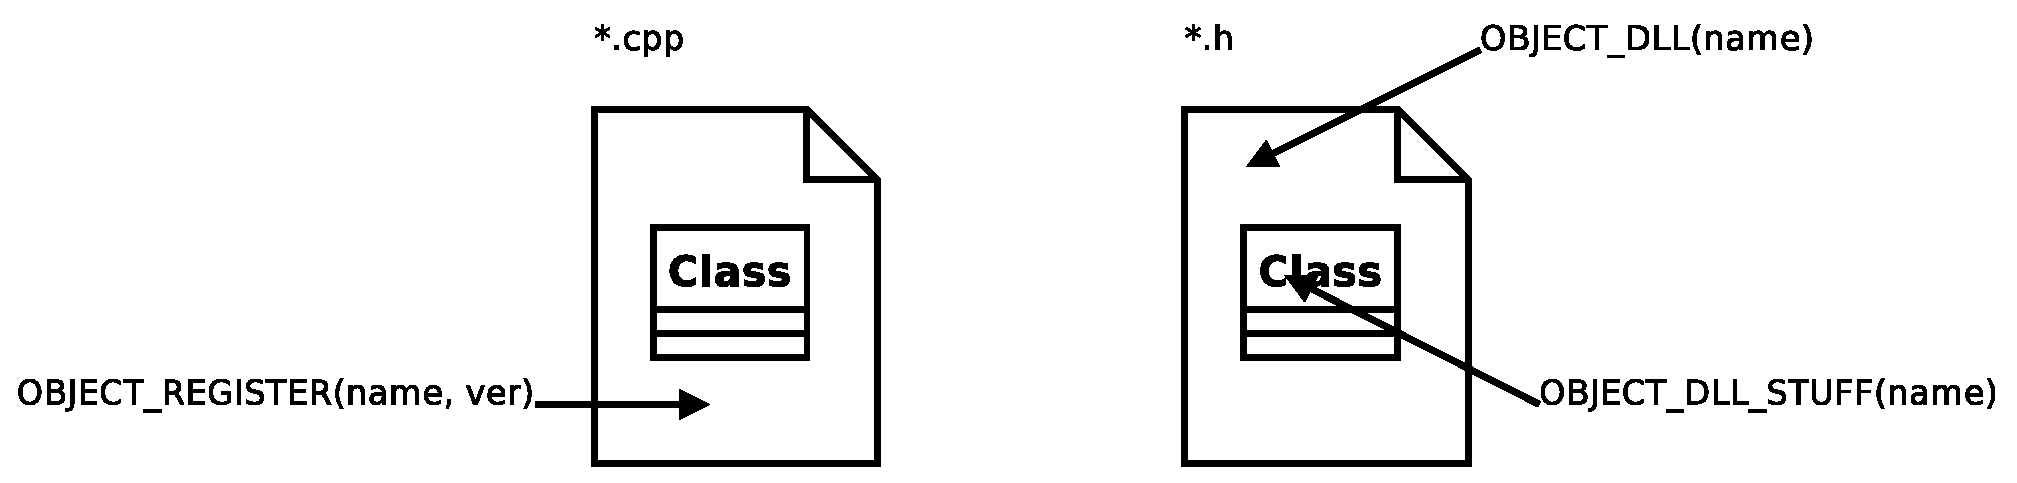
\includegraphics[width=0.77\textwidth]{level1/objectMacros.eps}
  \caption{BaseLib Level1 Object Macros position}
  \label{f:level1:object_macro}
 \end{center}
\end{figure}

The first two macros presented expand to the following code. That code redefine the class \texttt{new} and \texttt{delete} operators, provide a \texttt{Info} methods that return a \texttt{ObjectRegistryItem*} about that inform about the class type.

\begin{lstlisting}[
extendedchars=true,%
basicstyle=\fontfamily{pcr}\fontseries{m}\selectfont\footnotesize, %
stepnumber=1,%
numberstyle=\tiny,%
keywordstyle=\footnotesize\tt ,%
language=C++]
   extern "C" {
      ObjectRegistryItem* Get_private_ObjectInfo();
   }

class Object {
public:
   virtual ObjectRegistryItem* Info() const {
      return Get_private_ObjectInfo();
   }
   static void operator delete(void* p) {
      OBJDeleteFun(p,Get_private_ObjectInfo());
   }
   static void* operator new(unsigned int len) {
      return OBJNewFun(len,Get_private_ObjectInfo());
   }
   friend Object* ObjectBuildFn__ ();
\end{lstlisting}

Last macro listed expand to the following code that it is possible to find in the \texttt{*.cpp} file and is statically compiled one time. The first three row statically declare an \texttt{ObjectRegistryItem} that will be registered in the ORDB providing type information with the version information.

\begin{lstlisting}[
extendedchars=true,%
basicstyle=\fontfamily{pcr}\fontseries{m}\selectfont\footnotesize, %
stepnumber=1,%
numberstyle=\tiny,%
keywordstyle=\footnotesize\tt ,%
language=C++]
   static ObjectRegistryItem _private_ObjectInfo(Object,
      "$Id: level1.tex,v 1.12 2009/10/16 16:45:22 abarb Exp $",
      ObjectClassOffset(Object));
   ObjectRegistryItem *Get_private_ObjectInfo(){
      return &_private_ObjectInfo;
   }
\end{lstlisting}

There are also other macros in the \textit{level1/ObjectMacros.h} and are listed below. Comments are from the source code.

\begin{itemize}
\item \texttt{OBJECT\_DLL(name)} To allow registering a class contained in a DLL. Use before the class declaration outside the class
\item \texttt{OBJECT\_DLL\_STUFF(name)} To allow registering a class contained in a DLL. Use inside the class remember to set the public/private/protected afterwards.
\item \texttt{OBJECT\_STUFF(name)} To allow registering a class. Use inside the class. remember to set the public/private/protected afterwards.

\item \texttt{OBJECTREGISTER(name,ver)} Register a class with its version. Use in the \texttt{*.cpp} file
\item \texttt{OBJECTLOADREGISTER(name,ver)} Register a class with its version. Use in the \texttt{*.cpp} file. Automatically creates the Build function.
\item \texttt{OBJECTLOADREGISTERFLAGS(name,ext,flags,ver)} Register a class with its version. Use in the \texttt{*.cpp} file. Automatically creates the Build function. Sets the flags an the file extension.

\item \texttt{STRUCTREGISTER(name,structure)} Register a structure with its fields (structure). Use in the \texttt{*.cpp} file.

\item \texttt{BASICTYPEREGISTER(name,type)} Register a basic type (int float ...). Use in the \texttt{*.cpp} file.
\item \texttt{BASICTYPEREGISTER2(mod,name,type)} Register a basic type with a modifier in the name (short int long a = t ...). Use in the \texttt{*.cpp} file.
\item \texttt{BASICTYPEREGISTER3(mod,mod2,name,type )} Register a basic type with 2 modifiers in the name (short int long b=t ...).   Use in the .cpp file.
\end{itemize}



\subsection{Remarks}
TODO \\
TODO \\
TODO \\
Spiegare come sfruttare la reflection per creare una classe creare una classe via nome.



\subsection{Design Notes}
This section highlighted the basic RTTI-like functionality that BaseLib provide to the user. The ORDB presented here is a simply linked list with searching functionality. The design was made without thinking about preformance but focusing on the usability. The ORDB is really like a database, every loaded component of BaseLib as soon is loaded in the system register all class type it has and then, accessing the ORDB one can find the class it want and through the CDB loading it with the help of the ORDB. \\


At this level there is no hierical information between classes stored. So for example there is no method that tell you if a \texttt{ObjectRegistryDataBase} is a \texttt{LinkedListHolder} or not. This hierical relationship must be showed from the ORDB this can help also for the garbage collection (is it implemented in the GODB?). \\


ObjectTool is not necessary as a class: it has only one attribute can be deleted or improved.\\


The idea of having basic types and structured types is a good choice. Union's are probebly not the best choice because are rarely used in Object Oriented languages. The best design choice is to create an abstract type and subclassing it by basic types and by structured object: this is OOP (Object Oriented Programming).



\section{Global Object DataBase}
Such section address the \textit{Global Object Database} that mantain a list of all instantiated objects that registrates with them. A garbage collector mechanisms is implemented, each object that inherits from some other that is GarbageCollectable can be handled by the collector and make your work memory safe; every object that will be registered will be automatically deleted by the library, like in Java. This helps the programmer providing a way to not waste memory.

\begin{figure}[h!]
 \begin{center}
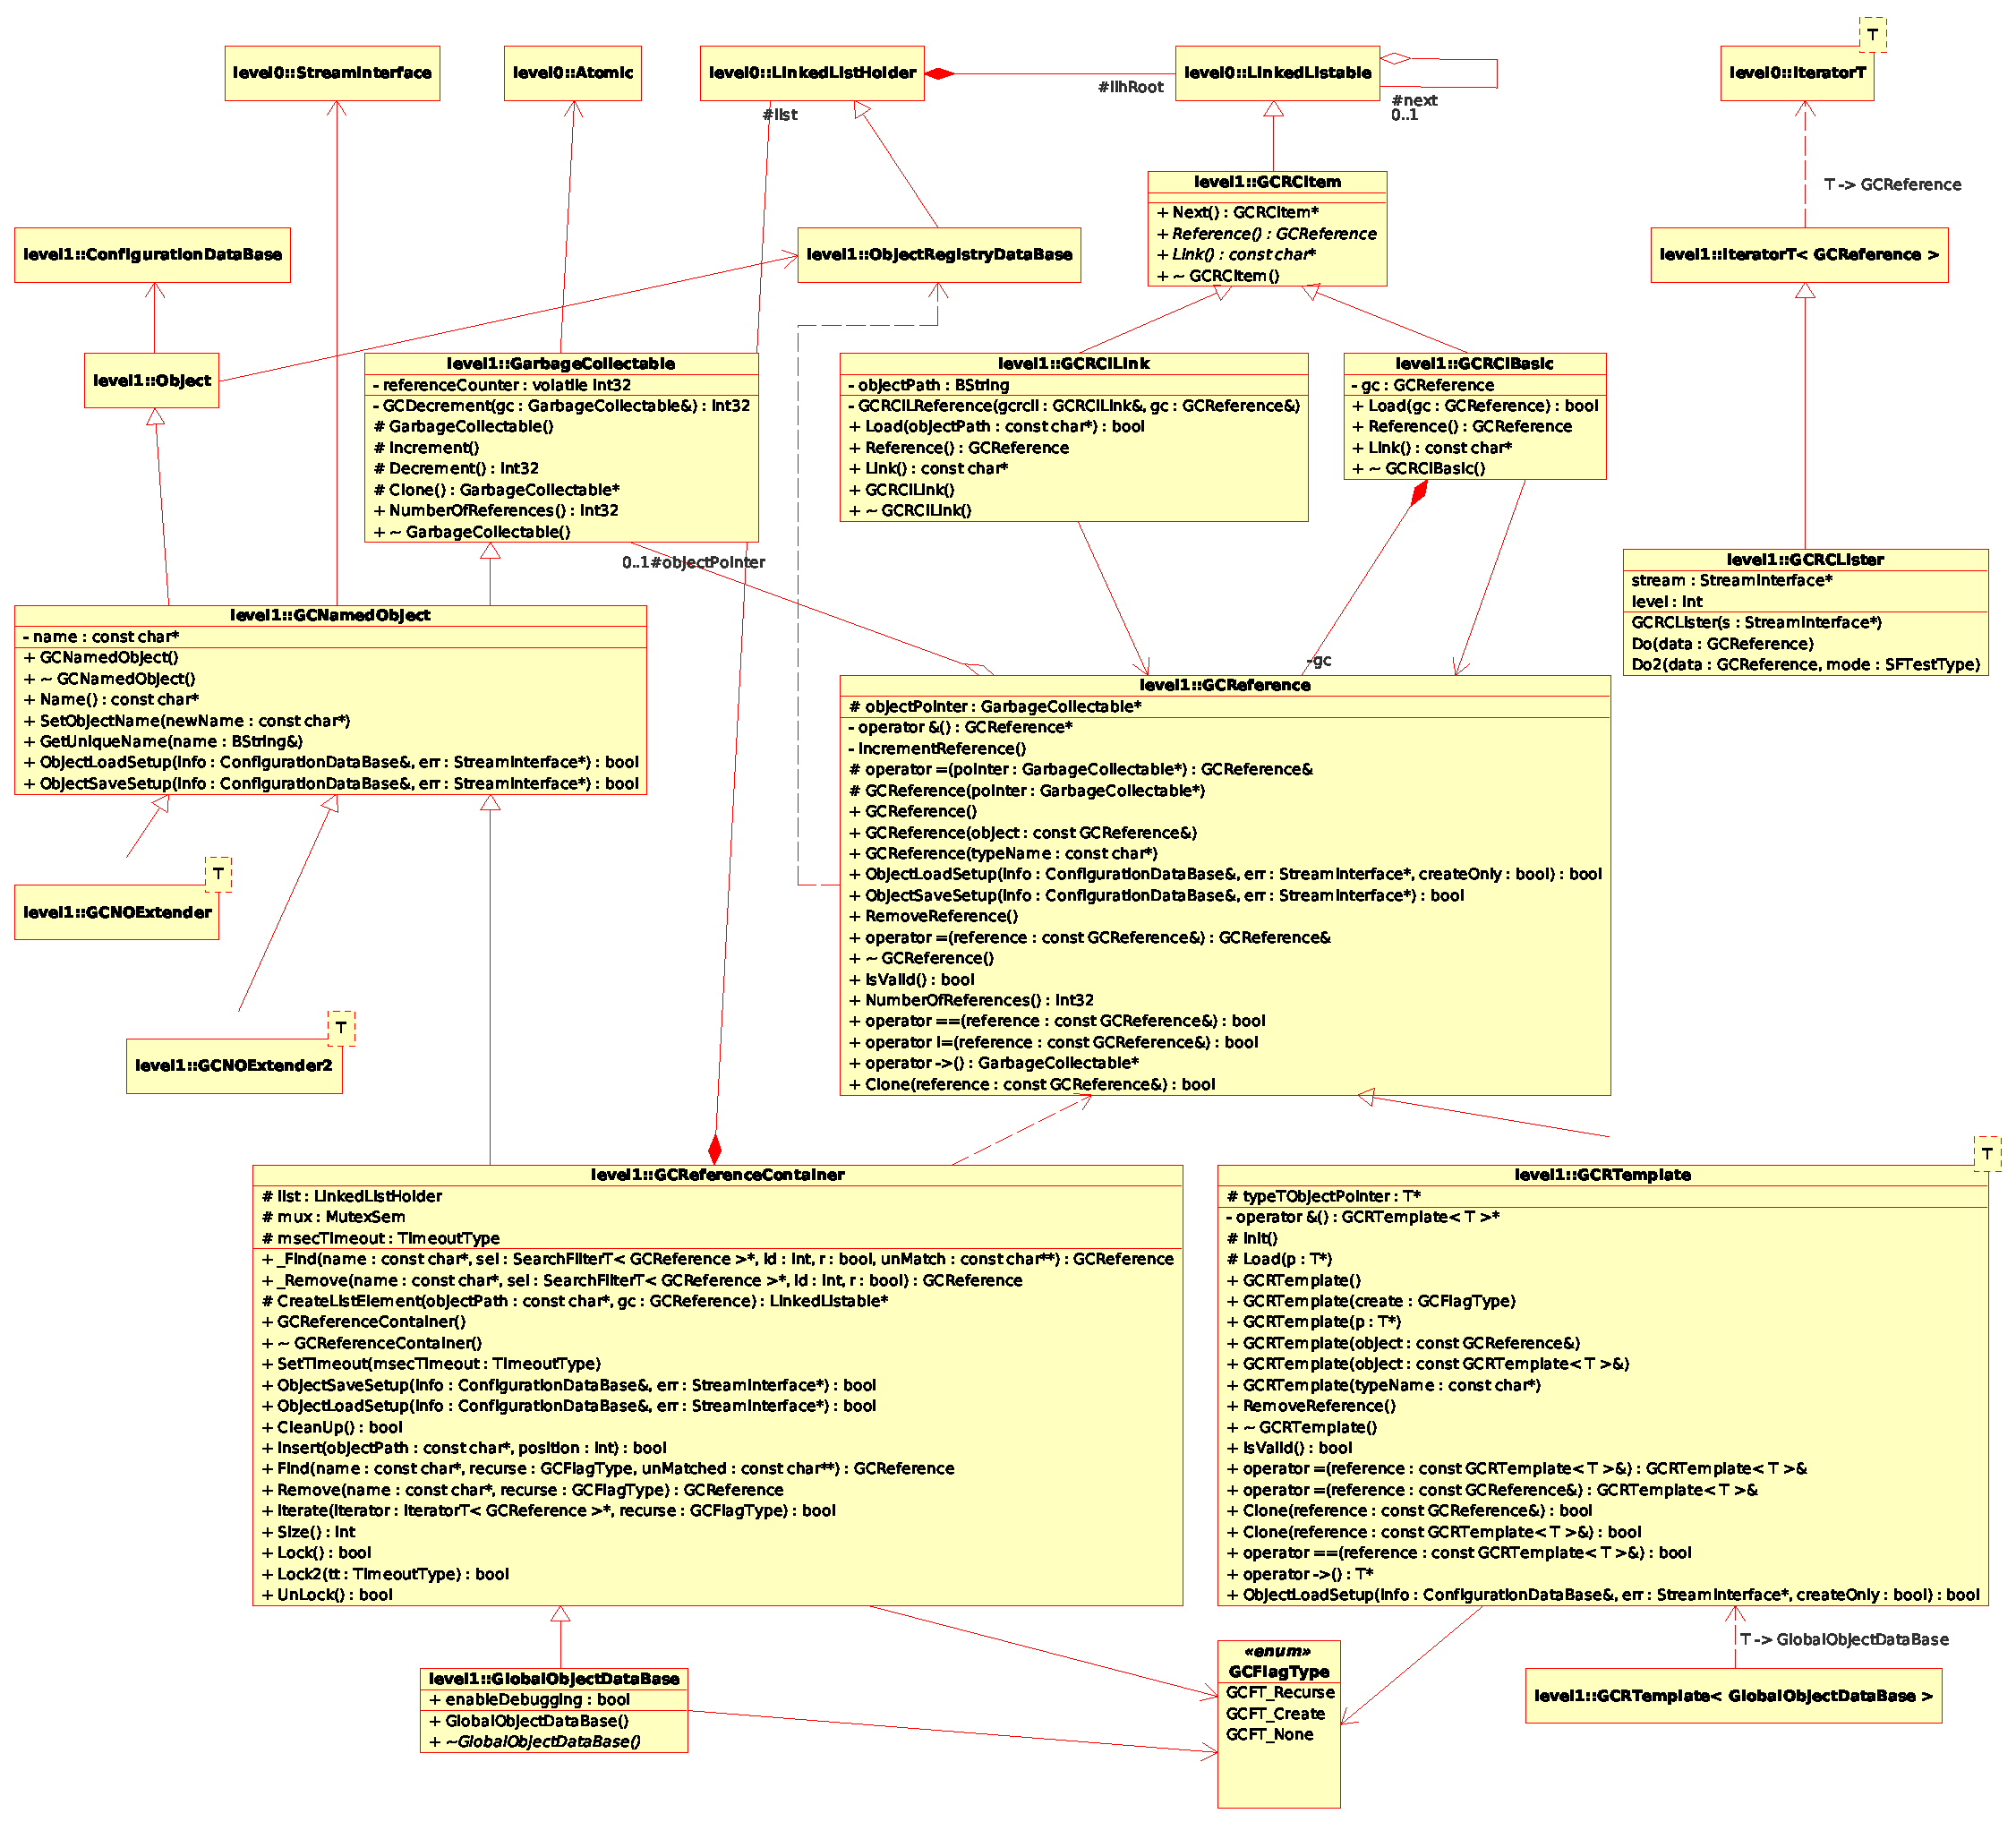
\includegraphics[width=1.1\textwidth]{level1/level1-GC.eps}
  \caption{BaseLib Level1 Global Object Database (GODB) classes}
  \label{f:level1:GC}
 \end{center}
\end{figure}

Objects of the class \texttt{GCNamedObject} inherits from \texttt{Object} but are also \texttt{GarbageCollectable}, so they are from a registered type in the ORDB but also can be collected for garbage reclaiming and within the \texttt{GCNamedObject} class they also have a name that is used to store different or the same object types in the GlobalObjectDataBase (GODB); in this way you can instantiate object by name and also reclaiming object.\\

What is the difference between an \texttt{Object} and an \texttt{GCNamedObject}? An \texttt{Object} registers in the ORDB a type of data, i.e. a class structure, a \texttt{GCNamedObject} instead register an instance of an object by name (or handle, or id). A \texttt{GCNamedObject} is also \texttt{GarbageCollectable} but an \texttt{Object} is not.\\

Classes in this section are depicted in the UML diagram of Figure \ref{f:level1:GC} and are listed below:

\begin{itemize}
 \item GarbageCollectable
 \item GCNamedObject
 \item GCNOExtender, GCNOExtender2

 \item GCRCItem, GCRCILink, GCRCIBasic
 \item GCRCLister
 \item GCReference

 \item GCRTemplate
 \item GCReferenceContainer
 \item GlobalObjectDataBase
\end{itemize}



\subsubsection{GarbageCollectable}
\texttt{[GarbageCollectable.h, GarbageCollectable.cpp]}\\
A class interface for implementing classes whose number of references is always accounted for; inherit from this class to implement garbage collection on a class. It accounts for reference to a class. It is really a simple class it provides only reference counting. \\


There is only one attribute \texttt{referenceCounter} that let supply all the functionality we need; the constructor initialises \texttt{referenceCounter} to zero, the method \texttt{Increment} is used to atomically increment the reference counter and the method \texttt{Decrement} is used to atomically decrement the reference counter.

To allow cloning of objects using references the final class must implement the method \texttt{Clone}. The method \texttt{NumberOfReferences} gets the number of references. The destructor is only called when the object is actually destroyed. The code does nothing here!

\begin{lstlisting}[
extendedchars=true,%
basicstyle=\fontfamily{pcr}\fontseries{m}\selectfont\footnotesize, %
stepnumber=1,%
numberstyle=\tiny,%
keywordstyle=\footnotesize\tt ,%
language=C++]
private:
   volatile int32 referenceCounter;
protected:
   GarbageCollectable();

   void Increment();
   int32 Decrement();

   virtual GarbageCollectable* Clone() const;
public:
   int32 NumberOfReferences() const;
   virtual ~GarbageCollectable();
\end{lstlisting}



\subsubsection{GCNamedObject}
\texttt{[GCNamedObject.h, GCNamedObject.cpp]}\\
A \texttt{GCNamedObject} is an extension of the \texttt{Object} class to include garbage collection and naming. It is used later to store object in the \texttt{GlobalObjectDataBase}.

A \texttt{GCNamedObject} is an \texttt{Object}, so it's class type will be registered, and it is also garbage collectable, so also it's usage is supervised and if it is not used jet it will be eliminated.\\


There is only one attribute \texttt{name} that adds to the \texttt{Object} a name string that will be necessary to identify it and so it must always contains a valid pointer to allocated memory. The constructor initialise to no name and the destructor deallocates memory.
The method \texttt{Name} accesses the name, \texttt{SetObjectName} sets the name and \texttt{GetUniqueName} returns a name that contains also the address, it begins with \textit{(address)name}.

The method \texttt{ObjectLoadSetup} initialises the name of the object using a CDB object, if \texttt{Name} is found than the name is taken from there, if missing then the \texttt{nodeName} is used, if \texttt{nodeName} start with \texttt{+} then the\texttt{ +} is removed (after reading the stuff about CDB you will better understand those comments). \texttt{ObjectSaveSetup} saves the settings in the CDB passed by argument.

\begin{lstlisting}[
extendedchars=true,%
basicstyle=\fontfamily{pcr}\fontseries{m}\selectfont\footnotesize, %
stepnumber=1,%
numberstyle=\tiny,%
keywordstyle=\footnotesize\tt ,%
language=C++]
private:
   const char* name;
public:
   GCNamedObject();
   virtual ~GCNamedObject();

   const char* Name()const;
   void SetObjectName(const char* newName);
   void GetUniqueName(BString& name);

   virtual bool ObjectLoadSetup(ConfigurationDataBase& info,
      StreamInterface* err);
   virtual bool ObjectSaveSetup(ConfigurationDataBase& info,
      StreamInterface* err);
\end{lstlisting}



\subsubsection{GCNOExtender, GCNOExtender2}
\texttt{[GCNOExtender.h]}\\
The following templates creates classes that are joint \texttt{GCNamedObject} and user defined class, used to add \texttt{GarbageCollection} and naming to existing classes. The first template is really simple: it creates a new class that inherits from \texttt{GCNamedObject} and the templatized class without adding any method.

\begin{lstlisting}[
extendedchars=true,%
basicstyle=\fontfamily{pcr}\fontseries{m}\selectfont\footnotesize, %
stepnumber=1,%
numberstyle=\tiny,%
keywordstyle=\footnotesize\tt ,%
language=C++]
template <class T>
class GCNOExtender: public GCNamedObject, public T
{
public:

};
\end{lstlisting}

The second template make the new class extending \texttt{GCNamedObject} and the templatized class as before but adds a redefinition of the methods \texttt{delete} and \texttt{new}.

\begin{lstlisting}[
extendedchars=true,%
basicstyle=\fontfamily{pcr}\fontseries{m}\selectfont\footnotesize, %
stepnumber=1,%
numberstyle=\tiny,%
keywordstyle=\footnotesize\tt ,%
language=C++]
template <class T>
class GCNOExtender2: public GCNamedObject, public T
{
public:
   static void operator delete(void* p){
      T::operator delete(p);
   }
   static void* operator new (unsigned int len){
      return T::operator new(len);
   }
};
\end{lstlisting}

Those templates are rarely used in the whole BaseLib (in BaseLib version 2 they are used only 2 times, one time in \textit{level1} and one time in \textit{level5}), probably are to be considered new stuff.



\subsubsection{GCRCItem, GCRCIBasic, GCRCILink}
\texttt{[GCRCItem.h]}\\
Classes that follow are all subclasses of the class \texttt{LinkedListable}. Such elements are used to store references in the references containers.

\paragraph{GCRCItem}
The class \texttt{GCRCItem} is not an interface, because has the \texttt{Next} method implemented, like an interface it also has no attributes. It is an abstract class for container of references. It requires to implements only a few simple methods that will complete the \texttt{LinkedListable} interface; \texttt{Next} gets next element skipping no \texttt{GCRCItem} derivatives; it has two virtual methods: \texttt{Reference} and \texttt{Link} that give you access to the object reference and to the link.

\begin{lstlisting}[
extendedchars=true,%
basicstyle=\fontfamily{pcr}\fontseries{m}\selectfont\footnotesize, %
stepnumber=1,%
numberstyle=\tiny,%
keywordstyle=\footnotesize\tt ,%
language=C++]
public:
   GCRCItem* Next();
   virtual GCReference Reference() = 0;
   virtual const char* Link() = 0;

   virtual ~GCRCItem(){};
\end{lstlisting}

\paragraph{GCRCIBasic}
The basic implementation of an abstract class \texttt{GCRCItem} is done by the class \texttt{GCRCIBasic}. It simply implements the two virtual methods above, i.e. \texttt{Reference} and \texttt{Link}; the method \texttt{Link} return \texttt{NULL}. There is a new method \texttt{Load} that let you set the class's attribute \texttt{gc}. The attribute is of type \texttt{GCReference} that is address in the next subsections.

\begin{lstlisting}[
extendedchars=true,%
basicstyle=\fontfamily{pcr}\fontseries{m}\selectfont\footnotesize, %
stepnumber=1,%
numberstyle=\tiny,%
keywordstyle=\footnotesize\tt ,%
language=C++]
private:
   GCReference gc;
public:
   bool Load(GCReference gc);
   virtual GCReference Reference();
   virtual const char* Link();

   virtual ~GCRCIBasic();
\end{lstlisting}

\paragraph{GCRCILink}
A \texttt{GCRCILink} object is a soft link to an object. It defines the same method as a \texttt{GCRCIBasic} but the \texttt{Load} method as a \texttt{const char*} argument instead of a \texttt{GCReference}. There is only one attribute of type \texttt{level0::BString}. The method \texttt{Link} return the attribute \texttt{objectPath}.

\begin{lstlisting}[
extendedchars=true,%
basicstyle=\fontfamily{pcr}\fontseries{m}\selectfont\footnotesize, %
stepnumber=1,%
numberstyle=\tiny,%
keywordstyle=\footnotesize\tt ,%
language=C++]
private:
   BString objectPath;
public:
   bool Load(const char* objectPath);
   virtual GCReference Reference();
   virtual const char* Link();

   GCRCILink();
   virtual ~GCRCILink();
\end{lstlisting}



\subsubsection{GCReference}
\texttt{[GCReference.h, GCReference.cpp]}\\
A class managing a pointer to an \texttt{Object} of type \texttt{GarbageCollectable}. The class implements a garbage collection mechanism that will destroy a class only when all references are destroyed. Access to the methods of the referred object is obtained via the \texttt{()} operator. Shared use of the same reference on multiple threads (static) needs semaphore protection. Use of different references to same object is safe. The only attribute of the class is a pointer to a \texttt{GarbageCollectable} object, that is private.

\begin{lstlisting}[
extendedchars=true,%
basicstyle=\fontfamily{pcr}\fontseries{m}\selectfont\footnotesize, %
stepnumber=1,%
numberstyle=\tiny,%
keywordstyle=\footnotesize\tt ,%
language=C++]
protected:
   GarbageCollectable* objectPointer;
\end{lstlisting}

We now explore the differents methods of the class. The first method, that is an operator overloading is like that to prevent users to make a copy of a reference by taking its address. The method \texttt{IncrementReference} allow to increment the usage count of the instantiated object. \\


Then follow a group of constructors and some copy constructors. The first two methods create a new \texttt{GCReference} object accepting a \texttt{GarbageCollectable} object pointer as an argument. Next constructor creates an empty reference, the other one creates a new reference from an existing one. The last constructor creates a new object of tyepe \texttt{typeName} and builds a reference to it. This is done by searching the \textit{Object Registry Database} for the class by name.

\begin{lstlisting}[
extendedchars=true,%
basicstyle=\fontfamily{pcr}\fontseries{m}\selectfont\footnotesize, %
stepnumber=1,%
numberstyle=\tiny,%
keywordstyle=\footnotesize\tt ,%
language=C++]
private:
   GCReference* operator&();
   void IncrementReference();

protected:
   GCReference(GarbageCollectable* pointer);
   GCReference& operator=(GarbageCollectable* pointer);
public:
   GCReference();
   GCReference(const GCReference& object);
   GCReference(const char* typeName);
   GCReference& operator=(const GCReference& reference);
\end{lstlisting}

In the last sections of this chapter we will look at the basics of what a \textit{Configuration Database} is. For now just think at a \texttt{Configuration Database} as a configuration file like \texttt{*.ini} file in MS Windows or any file in the \textit{/etc/} UNIX directory. \\


We now introduce some piece of such configuration files that enable the cretion of objects using that files via the class \texttt{GCReference}. The method \texttt{ObjectLoadSetup} that is the same we have seen in the \texttt{Object} class, it is not an overloading because \texttt{GCReference} doesn't inherits from any other class. 
Below is shown how to write a snippets of configuration file to create a class by name.
\begin{lstlisting}[
extendedchars=true,%
basicstyle=\fontfamily{pcr}\fontseries{m}\selectfont\footnotesize, %
stepnumber=1,%
numberstyle=\tiny,%
keywordstyle=\footnotesize\tt ,%
language=bash]
   Name = {
      Class = <class Name>
      <Class specific>
   }
\end{lstlisting}

A name can also be a linK to an object in the \textit{Global Object Database}. To load and save objects via a configuration file you need the methods \texttt{ObjectLoadSetup} and \texttt{ObjectSaveSetup}.

\begin{lstlisting}[
extendedchars=true,%
basicstyle=\fontfamily{pcr}\fontseries{m}\selectfont\footnotesize, %
stepnumber=1,%
numberstyle=\tiny,%
keywordstyle=\footnotesize\tt ,%
language=C++]
   virtual bool ObjectLoadSetup(ConfigurationDataBase& info,
             StreamInterface* err,
             bool createOnly=False);
   virtual bool ObjectSaveSetup(ConfigurationDataBase& info,
             StreamInterface * err);
\end{lstlisting}

The method \texttt{IsValid} estabilishes if the reference is pointing to a valid object or not; the method \texttt{NumberOfReference } gets the number of references the \texttt{GCReference} object holds. Follow some operator redefinitions. Then come the \texttt{Clone} method that creates a reference to a duplicate object; this is necessary, otherwise when \texttt{GCReference::Clone} is called by \texttt{GCRTemplate}, at this point the \texttt{IsValid} function of \texttt{GCRTemplate} would be called, returning false as the setup of \texttt{GCRTemplate} templatized object is not yet done.
The method \texttt{RemoveReference} correctly removes the reference. The distructor simply call this last function. If the reference count goes to zero the object will be destructed.

\begin{lstlisting}[
extendedchars=true,%
basicstyle=\fontfamily{pcr}\fontseries{m}\selectfont\footnotesize, %
stepnumber=1,%
numberstyle=\tiny,%
keywordstyle=\footnotesize\tt ,%
language=C++]
   virtual bool IsValid() const;
   inline int32 NumberOfReferences() const;

   inline bool operator==(const GCReference& reference) const;
   inline bool operator!=(const GCReference& reference) const;
   inline GarbageCollectable* operator->() const;

   inline bool Clone(const GCReference &reference);
   virtual void RemoveReference();

   virtual ~GCReference();
\end{lstlisting}



\subsubsection{GCRTemplate}
\texttt{[GCRTemplate.h]}\\
Definition of the widely used \texttt{GCRTemplate} class. This is a subclass of the \texttt{GCReference} class and it provides method overriding. Infact most of the \texttt{GCReference} methods are overriden. This template generates a specialised \texttt{GCReference} that is able to refer to objects of class \texttt{T} derivates.\\


\texttt{A \texttt{GCRTemplate} is an holder of a reference to an object. It helps garbage collection by increment and decrement the object usage count.} \\


The template class has only one (protected) attribute of type we are templatized for, called \texttt{typeTObjectPointer}.
\begin{lstlisting}[
extendedchars=true,%
basicstyle=\fontfamily{pcr}\fontseries{m}\selectfont\footnotesize, %
stepnumber=1,%
numberstyle=\tiny,%
keywordstyle=\footnotesize\tt ,%
language=C++]
protected:
   T* typeTObjectPointer;
\end{lstlisting}

We now skip operator redefinitions and we analize only other methods. The method \texttt{Init} simply sets all the class and superclass attributes to null values; the method \texttt{Load} first call \texttt{Init} and then using the argument passed by sets the class attibutes (\texttt{objectPointer} and \texttt{typeTObjectPointer}). \\


The first constructor coming is the default constructor and it simply call \texttt{Init}; the next constructor creates an empty reference or a reference to base type \texttt{T}, if argument \texttt{create} has value \texttt{GCFT\_CreateInstance} then it will also create the object (of type \texttt{T}).

The third constructor creates a reference to an object descendent from base type \texttt{T}. Recommended usage is \texttt{GCRTemplate<T>(new MYClass())}.

Fourth constructor creates a new reference copting from a generic one, the operation might fail, in which case the reference produced is invalid. The user has no feedback to understand if the operation was done with success or not, so it must test the object calling the \texttt{IsValid} method. This operation is done via the \texttt{operator=} that use the \texttt{dynamic\_cast} operator.

Next constructor creates a new reference from an existing one and the last one creates a new reference to an object spcified by name (via \texttt{typeName} argument).
\begin{lstlisting}[
extendedchars=true,%
basicstyle=\fontfamily{pcr}\fontseries{m}\selectfont\footnotesize, %
stepnumber=1,%
numberstyle=\tiny,%
keywordstyle=\footnotesize\tt ,%
language=C++]
template<typename T>
class GCRTemplate : public GCReference{
private:
   GCRTemplate<T>* operator&();
protected:
   void Init();
   void Load(T *p);

public:
   GCRTemplate();
   GCRTemplate(GCFlagType create);
   GCRTemplate(T *p);
   GCRTemplate(const GCReference& object);
   GCRTemplate(const GCRTemplate<T>& object);
   GCRTemplate(const char* typeName): GCReference(typeName);

   GCRTemplate<T>& operator=(const GCRTemplate<T>& reference);
   GCRTemplate<T>& operator=(const GCReference& reference);
\end{lstlisting}

Some overridden methods comes now; it is really interesting that each different class that can be loaded from a configuration file need to override the \texttt{ObjectLoadSetup} method to personalize its initialization beacuse each object needs its own params. \texttt{IsValid} estabilish if the reference is pointing to a valid object. In the same way \texttt{Clone} methods and the \texttt{RemoveReference} act as before but are specific for the subclass.

\begin{lstlisting}[
extendedchars=true,%
basicstyle=\fontfamily{pcr}\fontseries{m}\selectfont\footnotesize, %
stepnumber=1,%
numberstyle=\tiny,%
keywordstyle=\footnotesize\tt ,%
language=C++]
   virtual bool ObjectLoadSetup(ConfigurationDataBase& info,
                   StreamInterface* err,
                   bool createOnly=False);

   virtual bool IsValid() const;

   bool operator== (const GCRTemplate<T>& reference);
   T* operator->()const;

   inline bool Clone(const GCReference& reference);
   inline bool Clone(const GCRTemplate<T>& reference);
   virtual void RemoveReference();

   virtual ~GCRTemplate();
\end{lstlisting}



\subsubsection{GCReferenceContainer}
\texttt{[GCReferenceContainer.h, GCReferenceContainer.cpp]}\\

A \texttt{GCReferenceContainer} is a container (a list) of objects that are \texttt{GarbageCollectable}. If the object are also descendent from \texttt{GCNamedObject} then they can be accessed also by name.\\


The most important attribute in this class is the \texttt{list} it holds all objects contained by the conteiner. Other two attributes are a semaphore and the associated timeout, those attribute lets the access to the object be in an ordinate fashion to achieve data consistency.
\begin{lstlisting}[
extendedchars=true,%
basicstyle=\fontfamily{pcr}\fontseries{m}\selectfont\footnotesize, %
stepnumber=1,%
numberstyle=\tiny,%
keywordstyle=\footnotesize\tt ,%
language=C++]
protected:
   LinkedListHolder list;

   MutexSem mux;
   TimeoutType msecTimeout;
\end{lstlisting}

The method \texttt{CreateListElement} creates a new \texttt{GCRCILink} or \texttt{GCRCIBasic} object depending if the argument \texttt{objectPath} passed by is filled in or not. \texttt{SetTimeout} sets the internal semaphore timeout in msec. Methods \texttt{Lock} and \texttt{Lock2} lock the resource, must be unlocked using \texttt{UnLock} method.

\begin{lstlisting}[
extendedchars=true,%
basicstyle=\fontfamily{pcr}\fontseries{m}\selectfont\footnotesize, %
stepnumber=1,%
numberstyle=\tiny,%
keywordstyle=\footnotesize\tt ,%
language=C++]
protected:
   LinkedListable* CreateListElement(const char* objectPath,GCReference gc);
public:
   GCReferenceContainer();
   virtual ~GCReferenceContainer();
   void SetTimeout(TimeoutType msecTimeout);

   bool Lock();
   bool Lock2(TimeoutType tt)
   bool UnLock()

   virtual bool ObjectSaveSetup(ConfigurationDataBase& info,StreamInterface* err);
   virtual bool ObjectLoadSetup(ConfigurationDataBase& info,StreamInterface* err);
\end{lstlisting}

We have just mentioned the last two methods, \texttt{ObjectSaveSetup} and \texttt{ObjectLoadSetup}, such two are involved in  configuration and self instantiation of classes. We now explore the syntax of the accepted configuration parameters of the \texttt{GCReferenceContainer}. The basic syntax then follow, valid \texttt{<command>} are \texttt{Add}, \texttt{Remove}, and \texttt{AddReference}.
\begin{lstlisting}[
extendedchars=true,%
basicstyle=\fontfamily{pcr}\fontseries{m}\selectfont\footnotesize, %
stepnumber=1,%
numberstyle=\tiny,%
keywordstyle=\footnotesize\tt ,%
language=bash]
   <command> = {
      <command parameters>
   }
\end{lstlisting}

Imagine we want to add a new class of type \texttt{<name of class>} instantiated with the name \texttt{name1}, then we can write:

\begin{lstlisting}[
extendedchars=true,%
basicstyle=\fontfamily{pcr}\fontseries{m}\selectfont\footnotesize, %
stepnumber=1,%
numberstyle=\tiny,%
keywordstyle=\footnotesize\tt ,%
language=bash]
   Add = {
      name1 = {
         Class = <name of class>
         <class parameters>
      }
   }
\end{lstlisting}

A more easy way to do this is:
\begin{lstlisting}[
extendedchars=true,%
basicstyle=\fontfamily{pcr}\fontseries{m}\selectfont\footnotesize, %
stepnumber=1,%
numberstyle=\tiny,%
keywordstyle=\footnotesize\tt ,%
language=bash]
   +name1 = {
      Class = <name of class>
      <class parameters>
   }
\end{lstlisting}

To add a reference, i.e. to copy the reference from the \texttt{Global Object Database} of a class \texttt{name2} to a new instance called \texttt{name3} you have to write:

\begin{lstlisting}[
extendedchars=true,%
basicstyle=\fontfamily{pcr}\fontseries{m}\selectfont\footnotesize, %
stepnumber=1,%
numberstyle=\tiny,%
keywordstyle=\footnotesize\tt ,%
language=bash]
   AddReference = {
      name2 name3
   }
\end{lstlisting}

Removing an object can be done listing the named instances or by using special words like \texttt{ALL} below.

\begin{lstlisting}[
extendedchars=true,%
basicstyle=\fontfamily{pcr}\fontseries{m}\selectfont\footnotesize, %
stepnumber=1,%
numberstyle=\tiny,%
keywordstyle=\footnotesize\tt ,%
language=bash]
   Remove = {
      name1 name2 name3
   }
   Remove = {
      ALL
   }
\end{lstlisting}

After these few example with procede to finish to explore \texttt{GCReferenceContainer}'s methods. \\


The first \texttt{Insert} method adds an element at position \texttt{position}, the object added is a reference to the global object specified by \texttt{objectPath} argument; if \texttt{position} is \texttt{0} then the object is added before any other element, if is \texttt{-1} is added at the end of the list. The second \texttt{Insert} method adds an element at position \texttt{position} but now the object added is referenced to by \texttt{gc} that is a \texttt{GCReference} object pointer and contain the two arguments needed by the previous method.\\


The method \texttt{\_Find} is an helper method and is then called by the other following \texttt{Find} methods that we are going to explain. The first \texttt{Find} finds an object by \texttt{name} and returns a reference to it into \texttt{reference} argument; if \texttt{name} contains separators like \texttt{.} than the first segment is matched and the remainder is passed to the matching object if it is a container. If \texttt{recurse} is \texttt{true} and the pattern cannot be matched from the root then it will try searching also from the subnodes. The string tree is visited side to side. If \texttt{unMatched} is provided then a partial match is accepted and the unmatched part of the name is returned in \texttt{unMatched} as a pointer to name unmatched substring.

The second \texttt{Find} finds an object and returns a reference to it into \texttt{reference}, uses the \texttt{selector} \texttt{Test2} function (not \texttt{Test}) thus distinguishes between not found and not the right path and notifies of returning from recursion level using \texttt{SFTTBack}. One can match the partial finding on the way back out of recursion by returning \texttt{SFTTFound} in this last case.

The last \texttt{Find} gets a reference to the \texttt{index} -th element if \texttt{referenceAsBString} is \texttt{true} then a reference will be returned as a \texttt{BString}. \\


Like the method \texttt{\_Find} before there is a method \texttt{\_Remove} that is an helper method called by the following \texttt{Remove} methods. The first \texttt{Remove} method removes an object by \texttt{name} and returns a reference to it into \texttt{reference} argument. If \texttt{name} contains separators like \texttt{.} or \texttt{:} than the first segment is matched and the remainder is passed to the matching object if it is a container; if \texttt{recurse} is true then it will try searching also the subnodes.  The tree is visited side to side.

The second \texttt{Remove} removes any element from the list that fit the criteria specified by \texttt{selector}.

The last \texttt{Remove} removes the \texttt{index}-th element of the list. \\


The method \texttt{Cleanup} removes all references from the \texttt{GCReferenceContainer}. The method \texttt{Iterate} acts on each element of the list using the provided \texttt{iterator} if \texttt{recurse} is enabled it applies the \texttt{iterator} also on the sub containers after and before applying it on the container itself; note that this function does not keep the container locked during the call to the user function, when recursing, only the current container is locked. Last method, \texttt{Size} return the number of elements in the list.

\begin{lstlisting}[
extendedchars=true,%
basicstyle=\fontfamily{pcr}\fontseries{m}\selectfont\footnotesize, %
stepnumber=1,%
numberstyle=\tiny,%
keywordstyle=\footnotesize\tt ,%
language=C++]
   inline bool Insert(const char* objectPath,int position=-1);
   inline bool Insert(GCReference gc,int position=-1);

private:
   inline GCReference _Find(const char* name,SearchFilterT<GCReference>* selector=NULL,
            int index=-1,bool recurse=False,const char** unMatched=NULL);
public:
   inline GCReference Find(const char* name,GCFlagType recurse=GCFT_None,
            const char** unMatched=NULL)
   inline GCReference Find(SearchFilterT<GCReference>* selector,
            GCFlagType recurse=GCFT_None);
   inline GCReference Find(int index,bool referenceAsBString=False);

private:
   inline GCReference _Remove(const char* name,SearchFilterT<GCReference>* selector=NULL,
            int index=-1,bool recurse=False);
public:
   inline GCReference Remove(const char* name,GCFlagType recurse=GCFT_None);
   inline GCReference Remove(SearchFilterT<GCReference>* selector,
            GCFlagType recurse=GCFT_None);
   inline GCReference Remove(int index);

   inline bool CleanUp();
   bool Iterate(IteratorT<GCReference>* iterator,GCFlagType recurse=GCFT_None);
   int Size();
\end{lstlisting}



\subsubsection{GCRCLister}
\texttt{[GCReferenceContainer.h]}\\
Simply list (print) the content of a \texttt{GCReferenceContainer}. A \texttt{GCRCLister} is an \texttt{IteratorT<GCReference>} so it will handle \texttt{GCReference} objects that are linked listed in a \texttt{GCReferenceContainer}. Such a \texttt{GCRCLister} can be constructed only associating a \texttt{StreamInterface} object where to list all the elements founded in the \texttt{GCReferenceContainer}. The \texttt{StreamInterface} is also an attribute of the class, the other attribute, \texttt{level} account for the number of recursion levels. \\


The constructor require only one argument, if \texttt{s} is \texttt{NULL} the code will use \texttt{printf} to write to the console. Two \texttt{Do} methods do the work of listing.
\begin{lstlisting}[
extendedchars=true,%
basicstyle=\fontfamily{pcr}\fontseries{m}\selectfont\footnotesize, %
stepnumber=1,%
numberstyle=\tiny,%
keywordstyle=\footnotesize\tt ,%
language=C++]
   StreamInterface* stream;
   int level;
public:
   GCRCLister(StreamInterface* s = NULL);
   virtual void Do(GCReference data);
   virtual void Do2(GCReference data,SFTestType mode);
\end{lstlisting}



\subsubsection{GlobalObjectDataBase}
\texttt{[GlobalObjectDataBase.h, GlobalObjectDataBase.cpp]}\\

The \textit{Global Object Database} is statically declared as a
\begin{lstlisting}[
extendedchars=true,%
basicstyle=\fontfamily{pcr}\fontseries{m}\selectfont\footnotesize, %
stepnumber=1,%
numberstyle=\tiny,%
keywordstyle=\footnotesize\tt ,%
language=C++]
GCRTemplate<GlobalObjectDataBase> globalObjectDataBase;
\end{lstlisting}

in the file \textit{level1/GlobalObjectDataBase.cpp}. So the \textit{Global Object Database}, taking a look at Figure \ref{f:level1:GC} is a sort of template, templatizing with the class \texttt{GlobalObjectDataBase} that is of type \texttt{GCReferenceContainer}.\\


We explore first what a \texttt{GlobalObjectDataBase} class adds to a \texttt{GCReferenceContainer} type. The source follows.
\begin{lstlisting}[
extendedchars=true,%
basicstyle=\fontfamily{pcr}\fontseries{m}\selectfont\footnotesize, %
stepnumber=1,%
numberstyle=\tiny,%
keywordstyle=\footnotesize\tt ,%
language=C++]
class GlobalObjectDataBase: public GCReferenceContainer{
public:
   bool enableDebugging;
   GlobalObjectDataBase(){
      if (enableDebugging)
         DisplayRegisteredClasses(NULL,True);
   }
   virtual ~GlobalObjectDataBase(){
      if (enableDebugging)
         DisplayRegisteredClasses(NULL,True);
   }
};
\end{lstlisting}

A \texttt{GlobalObjectDataBase} class simply adds a debugging facility to a \texttt{GCReferenceContainer} class. Attribute \texttt{enableDebugging} enable or disable the debugging facility.

The \textit{Global Object Database}, \texttt{globalObjectDataBase}, is a \texttt{GCRTemplate} that subclass a \texttt{GCReference} and then contain a list of \texttt{GlobalObjectDataBase} elements.\\


The \textit{Global Object Database} is the default container of objects, every contained object could be addressed and indexed. When objects will be destroyed the virtualized destructor will be removed from the leafes.

Performs the job of destroying the database note that the global destructor is called in a single thread environment during the final winding down of an application for this reason there is no need to check for the database being in use that is the hope at least.



\subsection{Design Notes}
There is no hierical of the class saved, no inter relationship between classes is stored.



\section{Error System Instruction}
The \textit{Error System Instruction} (ESI) is a subset of the Error Management System (EMS) that create a linked list of errors and errors' behaviour of the system. All code is in header files and must be included in all files that needed Error Management.

\begin{figure}[h!]
 \begin{center}
  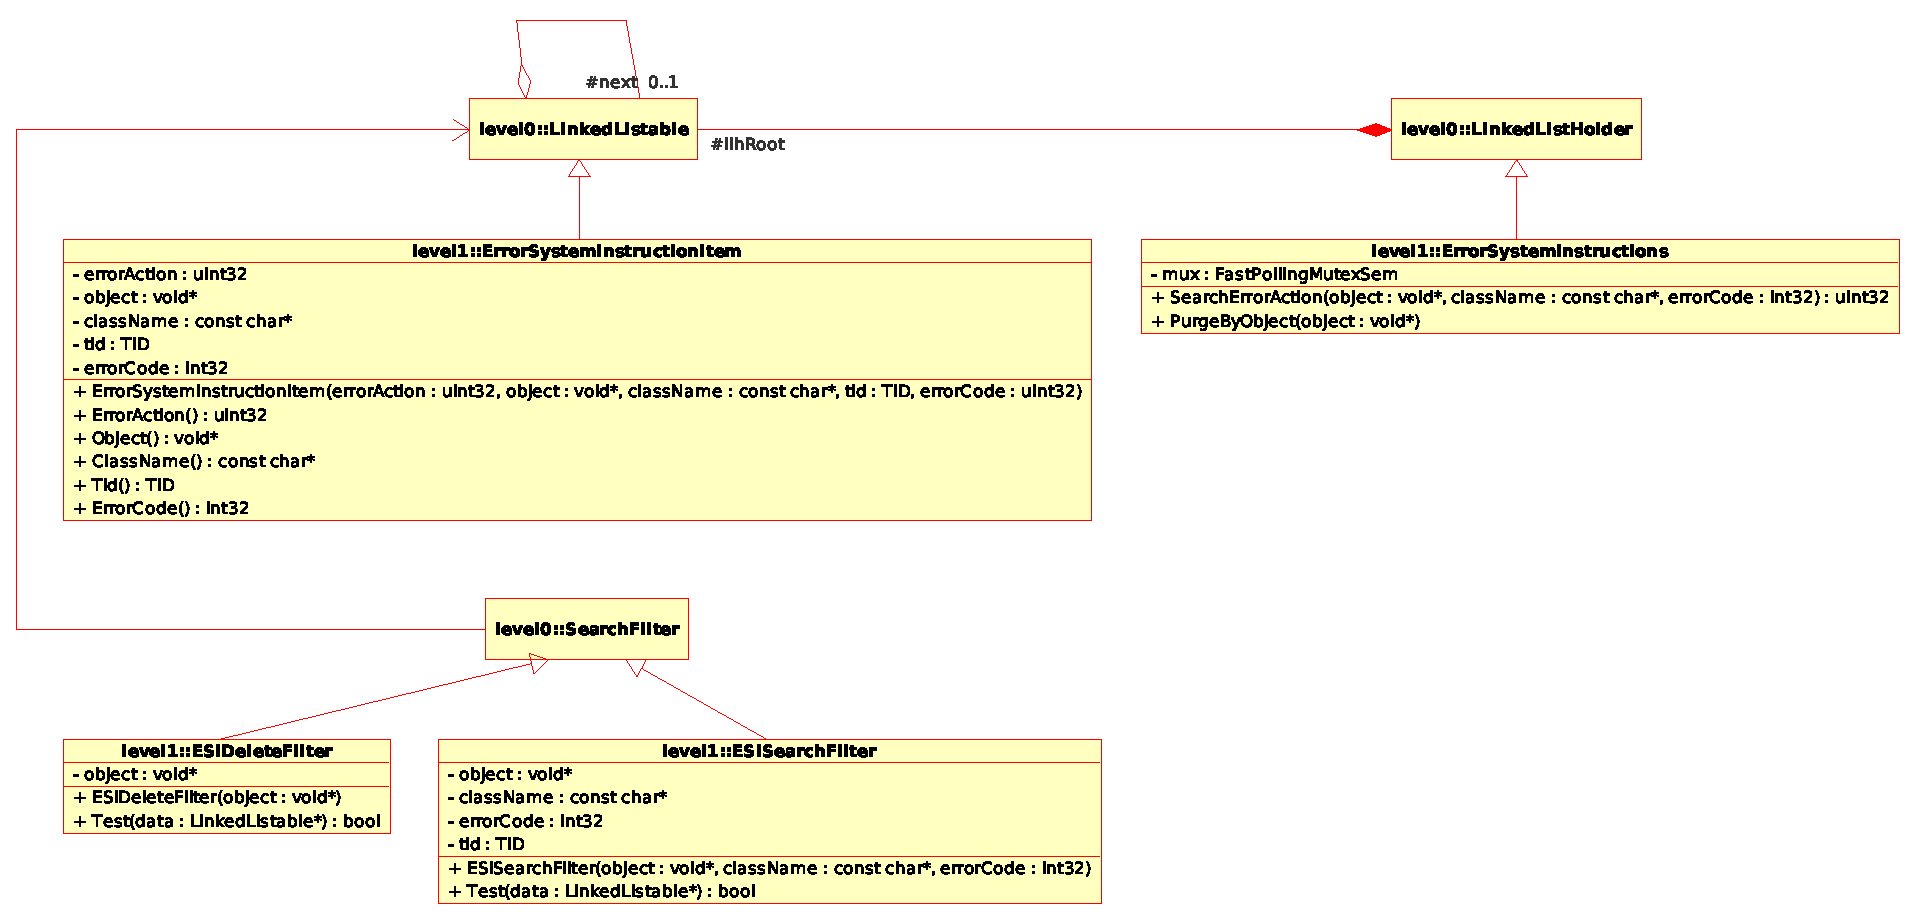
\includegraphics[width=\textwidth]{level1/level1-ESI.eps}
  \caption{BaseLib Level1 Error System Instruction classes}
  \label{f:level1:esi}
 \end{center}
\end{figure}

The UML diagram is depicted in Figure \ref{f:level1:esi} but if you look also to Figure \ref{f:level1:object} you can note that also \texttt{Object} relies on top of the ESI infrastructure; for each class type there is also an ESI item that decides what action to take in case of an error condition.\\

ESI is another linked listable structure that accounts about errors, i.e. is a catalog of errors and actions, classes involved in this level are:

\begin{itemize}
 \item ErrorSystemInstructionItem
 \item ErrorSystemInstructions
 \item ESIDeleteFilter, ESISearchFilter
\end{itemize}



\subsubsection{ErrorSystemInstructionItem}
\texttt{[ErrorSystemInstructionItem.h]}\\
The basic component of the ESI is the class \texttt{ErrorSystemInstructionItem}, there is a class like that for every error and basically tall the system what to do in case a specific error.

We start with the attributes, the first attribute, \texttt{errorAction}, tell the system what to do with this error, \texttt{object} is the address of the object the action is restricted to, attribute \texttt{className} is the name of class the action is restricted to, \texttt{tid} is the thread identification the action is restricted to and \texttt{errorCode} is the error code the action is restricted to. If you choose to not restrict error management to any of the previous attributes simply sets them to \texttt{NULL}.

The constructor lets you set the policy for an error, all the other methods let you get the attributes of the class.
\begin{lstlisting}[
extendedchars=true,%
basicstyle=\fontfamily{pcr}\fontseries{m}\selectfont\footnotesize, %
stepnumber=1,%
numberstyle=\tiny,%
keywordstyle=\footnotesize\tt ,%
language=C++]
   uint32 errorAction;
   void* object;
   const char* className;
   TID tid;
   int32 errorCode;
public:
   ErrorSystemInstructionItem(uint32 errorAction,
         void* object,
         const char* className,
         TID tid,
         int32 errorCode);
   uint32 ErrorAction();
   void* Object();
   const char* ClassName();
   TID Tid();
   int32 ErrorCode();
\end{lstlisting}

Some defined \texttt{ErrorSystemInstructionItem} in file \textit{level1/ErrorSystemInstructionItem.h}:
\begin{lstlisting}[
extendedchars=true,%
basicstyle=\fontfamily{pcr}\fontseries{m}\selectfont\footnotesize, %
stepnumber=1,%
numberstyle=\tiny,%
keywordstyle=\footnotesize\tt ,%
language=C++]
#define ANY_VALUE NULL

#define OBJECT_ERRORINSTRUCTION(errorAction,object,code) \
   new ErrorSystemInstructionItem(errorAction,object,ANY_VALUE,ANY_VALUE,code)
#define ERRCODE_ERRORINSTRUCTION(errorAction,code) \
   new ErrorSystemInstructionItem(errorAction,ANY_VALUE,ANY_VALUE,ANY_VALUE,code)
#define CLASS_ERRORINSTRUCTION(errorAction,classInfo,code) \
   new ErrorSystemInstructionItem(errorAction,ANY_VALUE,classInfo,ANY_VALUE,code)
#define TID_ERRORINSTRUCTION(errorAction,tid,code) \
   new ErrorSystemInstructionItem(errorAction,ANY_VALUE,ANY_VALUE,tid,code)
\end{lstlisting}



\subsubsection{ErrorSystemInstructions}
\texttt{[ErrorSystemInstructions.h]}\\
The class \texttt{ErrorSystemInstructions} is a collection of \texttt{ErrorSystemInstructionItem}s, i.e. a container of \texttt{ErrorSystemInstructionItem}: what to do in case of an error. It is a subclass of \texttt{LinkedListHolder}.

The only added attribute to the \texttt{LinkedListHolder} class is a \texttt{FastPollingMutexSem} that manages the access to the resources. The method \texttt{SearchErrorAction} searches using one of the three keys as arguments an method \texttt{PurgeByObject} remove the \texttt{ErrorSystemInstructionItem} associated to an object passed by pointer.
\begin{lstlisting}[
extendedchars=true,%
basicstyle=\fontfamily{pcr}\fontseries{m}\selectfont\footnotesize, %
stepnumber=1,%
numberstyle=\tiny,%
keywordstyle=\footnotesize\tt ,%
language=C++]
   FastPollingMutexSem mux;
public:
   uint32 SearchErrorAction(void *object,const char *className,int32 errorCode);
   void PurgeByObject(void *object);
\end{lstlisting}



\subsubsection{ESIDeleteFilter, ESISearchFilter}
\texttt{[ErrorSystemInstructions.h]}\\
Methods implemented in the previous \texttt{ErrorSystemInstructions} class work using the class defined in this section: \texttt{ESIDeleteFiler} and \texttt{ESISearchFilter}. The first one, \texttt{ESIDeleteFilter}, is a filter to delete \texttt{ErrorSystemInstructionItem}; and the last one, \texttt{ESISearchFilter}, searches for \texttt{ErrorSystemInstructionItem} by different criteria.



\section{Configuration Database}
The \textit{Configuration Database} (CDB) is one of the key concepts upon BaseLib is developed. There are not to many classes in this level concerning the CDB, infact its classes are spreaded across many levels. In this level the developer will find a sort of interface to CDB: the \texttt{CDBVirtual} abstract class that by the way can be considered as an interface but has one non pure virtual method.

In next levels we will face with three CDBs' implementations (CDB, CDBOS, MMCDB). If one want to go a bit further can write a CDB that parse XML file for example and make it work in the framework simply let it work observe the interface we are now discussing about in this section.

\begin{figure}[h!]
 \begin{center}
  \includegraphics[width=\textwidth]{level1/level1-CDB.eps}
  \caption{BaseLib Level1 Configuration Database classes}
  \label{f:level1:CDB}
 \end{center}
\end{figure}

Figure \ref{f:level1:CDB} depicts the UML diagram of the involved classes that are:
\begin{itemize}
 \item CDBVirtual
 \item CDBNull
 \item ConfigurationDataBase
\end{itemize}



\subsubsection{CDBVirtual}
\texttt{[CDBVirtual.h, CDBTypes.h]}\\
The class \texttt{CDBVirtual} provide an interface to a hierarchical database. It works similarly to a filesystem having directory nodes (branches) and file nodes (leaves). Each leaf node is a container of a sequence of characters, both ASCII and not ascii. CDB is infact a reference to an instance of the database. Copying CDBs does not duplicate the database but increases a reference counter. Operation to the same database by different threads is safe. The methods of this class are not usable directly outside BaseLib Use \texttt{CreateCDB} to create an instance of CDB. \\


Class \texttt{CDBVirtual} has many pure virtual methods, we go throught those. In the file \textit{level1/CDBTypes.h} all the enumeration used are can be founded.

The deconstructor will destroy database if instance count goes to zero. The method \texttt{Clone} creates a new reference to a database, or if that is not possible it creates a copy; \texttt{cdbcm=CDBCM\_CopyAddress} ensures that the new object points at the same location. The method \texttt{CleanUp} removes all the content from the database unless some other database instance exists and points to a subtree, one can reques to delete only the current subtree.
The method \texttt{Lock} locks the main database for exclusive access: use if a group of transactions should be atomic; \texttt{UnLock} unlocks the main database: remember to unlocking a locked database after useing it.
\begin{lstlisting}[
extendedchars=true,%
basicstyle=\fontfamily{pcr}\fontseries{m}\selectfont\footnotesize, %
stepnumber=1,%
numberstyle=\tiny,%
keywordstyle=\footnotesize\tt ,%
language=C++]
   virtual ~CDBVirtual();
   virtual CDBVirtual* Clone(CDBCreationMode cdbcm)=0;
   virtual void CleanUp(CDBAddressMode cdbam=CDBAM_FromRoot) = 0;
   virtual bool Lock() = 0;
   virtual void UnLock() = 0;
\end{lstlisting}

The method \texttt{SubTreeName} finds the overall path leading to the current node, return the path in the argument \texttt{name}, \texttt{NodeName} returns the name of the current node in \texttt{name}; \texttt{NodeType} return the type of the current node in \texttt{name}; the method \texttt{AddChildAndMove} can be used to create a new subtree.

The method \texttt{NumberOfChildren} tells how many branches from this node, negative number implies that the location is a leaf; \texttt{Move} moves to the specified location; the movement is relative to the current location, \texttt{UpNode} is one level up, \texttt{RootNode} is all the way up. The mehtod \texttt{MoveToChildren} lets you move in the tree, negative numbers move up, 0 is the first of the children and a positive number is the n-th children; \texttt{MoveToFather} let s you move in the tree, 0 means remain where you are, greater then 0 to brothers on the right below 0 on the left. The method \texttt{CopyFrom} and \texttt{CopyTo} copy from the CDB to another one. \texttt{MoveToRoot} moves back to the root of the tree.
The method \texttt{FindSubTree} searches on the right of the tree for the subtree identified by the string \texttt{configName}; on success nodes points to the node containing the subtree or leaf; it will not follow links; the only argument it supports is \texttt{CDBAM\_SkipCurrent} that allow a search in the current subtree excluding current node any other flag are NOT SUPPORTED.
The method \texttt{Size} gives the total number of nodes; argument can be \texttt{CDBAM\_SubTreeOnly} allowing to measure the current subtree, or \texttt{CDBAM\_LeafsOnly}   allowing counting only the data nodes. \texttt{TreePosition} returns the position of the node in the left to right bottom to top order the absolute location of a node; \texttt{CDBAM\_LeafsOnly} allows counting only the data nodes. The method \texttt{TreeMove} moves to a location within the whole (sub)tree; the nodes are numbered from left to right and from subnode to supernode; if the node does not exist returns False and remains in the start position.

\begin{lstlisting}[
extendedchars=true,%
basicstyle=\fontfamily{pcr}\fontseries{m}\selectfont\footnotesize, %
stepnumber=1,%
numberstyle=\tiny,%
keywordstyle=\footnotesize\tt ,%
language=C++]
   virtual bool SubTreeName(Streamable& name,const char* sep = ".") = 0;
   virtual bool NodeName(BString& name) = 0;
   virtual bool NodeType(BString& name) = 0;

   virtual bool AddChildAndMove(const char* subTreeName,
      SortFilterFn* sorter=NULL) = 0;
   virtual int  NumberOfChildren()=0;
   virtual bool Move(const char* subTreeName) = 0;
   virtual bool MoveToChildren(int childNumber=0) = 0;
   virtual bool MoveToBrother(int steps = 1) = 0;
   virtual bool MoveToFather(int steps = 1) = 0;
   virtual bool CopyFrom(CDBVirtual* cdbv) = 0;
   inline bool  CopyTo(CDBVirtual* cdbv);
   inline  bool MoveToRoot();

   virtual bool FindSubTree(const char* configName,
      CDBAddressMode cdbam=CDBAM_None)=0;
   virtual int  Size(CDBAddressMode cdbam) = 0;
   virtual int  TreePosition(CDBAddressMode cdbam=CDBAM_LeafsOnly) = 0;
   virtual bool TreeMove(int index,
      CDBAddressMode cdbam=CDBAM_LeafsOnly) = 0;
\end{lstlisting}

The method \texttt{GetArrayDims} if doesn't fail returns the \texttt{size}, \texttt{maxDim} and \texttt{configName} of the CDB. The method \texttt{ReadArray} read the array, if \texttt{size} is \texttt{NULL} it treats the input as a monodimensional array of size \texttt{nDim}, if \texttt{nDim} is zero this is a standard variable equivalent of a vector of size 1, if size does not agree with the actual dimensions of the matrix the routine will fail. We can tell the same for the \texttt{WriteArray} method.\\


The method \texttt{Delete} removes an entry or subtree (position is relative) to delete a link use the \texttt{linkTo} as the leaf name to delete a subtree simply specify the group node. The method \texttt{Exists} tell you whether a certain entry exists. The method \texttt{Link} make a link, \texttt{linkFrom} is the path where the link is created from.\\


The method \texttt{ReadFromStream} reads a database from a stream; \texttt{EnableParserReports} enables reports of parser during \texttt{ReadFromStream} into error stream. \texttt{WriteToStream} writes the database to stream without any ordering; \texttt{LoadFromEnvironment} loads from environment or from any \texttt{NULL} terminated list of chars.\\


The method \texttt{ReadStructure} read from CDB to memory and the method \texttt{WriteStructure} either copies or references a memory structure, at address \texttt{address} and of type \texttt{className} CDB transforms the memory.

\begin{lstlisting}[
extendedchars=true,%
basicstyle=\fontfamily{pcr}\fontseries{m}\selectfont\footnotesize, %
stepnumber=1,%
numberstyle=\tiny,%
keywordstyle=\footnotesize\tt ,%
language=C++]
   virtual bool GetArrayDims(int* size, int& maxDim, const char* configName,
      CDBArrayIndexingMode cdbaim=CDBAIM_Flexible) = 0;
   virtual bool ReadArray(void* array, const CDBTYPE& valueType,
      const int* size, int nDim, const char* configName) = 0;
   virtual bool WriteArray(const void* array, const CDBTYPE& valueType,
      const int* size, int nDim, const char* configName, 
      SortFilterFn* sorter=NULL) = 0;

   virtual bool Delete(const char* configName) = 0;
   virtual bool Exists(const char* configName) = 0;
   virtual bool Link(const char* linkFrom,
      const char* linkTo,
      SortFilterFn* sorter=NULL) = 0;

   virtual bool ReadFromStream(StreamInterface& stream,
      StreamInterface* err=NULL,SortFilterFn* sorter=NULL) = 0;
   virtual void EnableParserReports(bool flag) = 0;
   virtual bool WriteToStream(StreamInterface& stream,
      StreamInterface* err=NULL,CDBWriteMode mode=CDBWM_Tree) = 0;
   virtual bool LoadFromEnvironment(char** env) = 0;

   virtual bool ReadStructure (const char* className,
      char* address,
      Streamable* err=NULL) = 0;
   virtual bool WriteStructure(const char* className,
      char* address,
      const char* variableName=NULL,
      Streamable* err=NULL) = 0;
\end{lstlisting}



\subsubsection{CDBNull}
\texttt{[CDBNull.h]}\\
Class \texttt{CDBNull} is a dummy CDB just to create valid references. Each method is implemented returning zero or \texttt{False}.



\subsubsection{ConfigurationDataBase}
\texttt{[ConfiguratonDataBase.h]}\\
Differently from other data structures that we have founded during this chapter, like ORDB and GODB, you can instantiate how many \textit{Configuration Database}s you need and there is no static and globally defined CDB. A \texttt{ConfigurationDataBase} contains a reference to CDB of type \texttt{CDBVirtual} because it inherits from \texttt{GCRTemplate<CDBVirtual>}. Forces call to CDB to be made via the virtual table. \\


The method \texttt{Load} copy the \texttt{CDBVirtual} pointer in the \texttt{GCRTemplate} templatized attribute \texttt{typeTObjectPointer} after type checking. The first constructor
 creates a new database if \texttt{base} paramenter is \texttt{NULL}, if not \texttt{NULL} it creates a reference to an existing one. The second constructor creates a CDB from a generic base type.

\begin{lstlisting}[
extendedchars=true,%
basicstyle=\fontfamily{pcr}\fontseries{m}\selectfont\footnotesize, %
stepnumber=1,%
numberstyle=\tiny,%
keywordstyle=\footnotesize\tt ,%
language=C++]
protected:
   void Load(CDBVirtual *p);
public:
   inline ConfigurationDataBase(ConfigurationDataBase &base,
      CDBCreationMode cdbcm=CDBCM_CopyAddress);
   inline ConfigurationDataBase(const char* coreClassName="CDB");
   inline ConfigurationDataBase(GCReference cdb,
      CDBCreationMode cdbcm=CDBCM_CopyAddress);
   inline void operator=(ConfigurationDataBase &base);

   virtual  ~ConfigurationDataBase();
   CDBVirtual *operator->();
\end{lstlisting}



\subsection{Design Notes}
The class \texttt{ConfigurationDataBase} declared with all inline methods in \textit{level1/ConfigurationDataBase.h} is included in many BaseLib's files, this way the code will be compiled to many times wasting space. Class \texttt{CDBVirtual} looks so heavy could be stripped off?
